\documentclass[alpha-refs]{wiley-article}
\usepackage{amsmath}
\usepackage{graphicx}%
\usepackage{amsfonts}%
\usepackage{amssymb}
\RequirePackage[colorlinks,citecolor=blue,urlcolor=blue]{hyperref}
%\usepackage{natbib}
\usepackage{float}
\usepackage{subcaption}
%\usepackage[margin=1in]{geometry}
\allowdisplaybreaks
%\usepackage{amsthm}

%\usepackage{algorithm}% http://ctan.org/pkg/algorithms
%\usepackage{algpseudocode}% http://ctan.org/pkg/algorithmicx



\newcommand{\blam}{ \mbox{\boldmath $ \lambda $} }
\newcommand{\bet}{ \mbox{\boldmath $ \eta $} }
\newcommand{\bome}{ \mbox{\boldmath $ \omega $} }
\newcommand{\bbet}{ \mbox{\boldmath $ \beta $} }
\newcommand{\bbeta}{ \mbox{\boldmath $ \beta $} }
\newcommand{\balph}{ \mbox{\boldmath $ \alpha $} }
\newcommand{\balpha}{ \mbox{\boldmath $ \alpha $} }
\newcommand{\bphi}{ \mbox{\boldmath $\phi$}}
\newcommand{\bzeta}{ \mbox{\boldmath $\zeta$}}
\newcommand{\bkap}{ \mbox{\boldmath $\kappa$}}
\newcommand{\bkappa}{ \mbox{\boldmath $\kappa$}}
\newcommand{\beps}{ \mbox{\boldmath $\epsilon$}}
\newcommand{\bepsilon}{ \mbox{\boldmath $\epsilon$}}
\newcommand{\bthet}{ \mbox{\boldmath $ \theta $} }
\newcommand{\btheta}{ \mbox{\boldmath $ \theta $} }
\newcommand{\bnu}{ \mbox{\boldmath $\nu$} }
\newcommand{\bmu}{ \mbox{\boldmath $\mu$} }
\newcommand{\bOmega}{ \mbox{\boldmath $\Omega$} }
\newcommand{\bGam}{ \mbox{\boldmath $\Gamma$} }
\newcommand{\bSig}{ \mbox{\boldmath $\Sigma$} }
\newcommand{\bSigma}{ \mbox{\boldmath $\Sigma$} }
\newcommand{\bPhi}{ \mbox{\boldmath $\Phi$} }
\newcommand{\bThet}{ \mbox{\boldmath $\Theta$} }
\newcommand{\bTheta}{ \mbox{\boldmath $\Theta$} }
\newcommand{\bDel}{ \mbox{\boldmath $\Delta$} }
\newcommand{\bDelta}{ \mbox{\boldmath $\Delta$} }
\newcommand{\bnabla}{ \mbox{\boldmath $\nabla$} }
\newcommand{\bLam}{ \mbox{\boldmath $\Lambda$} }
\newcommand{\bLambda}{ \mbox{\boldmath $\Lambda$} }
\newcommand{\bLambdasub}{ \scriptsize{\bLambda}}
\newcommand{\bgam}{ \mbox{\boldmath $\gamma$} }
\newcommand{\bgamma}{ \mbox{\boldmath $\gamma$} }
\newcommand{\brho}{ \mbox{\boldmath $\rho$} }
\newcommand{\bdel}{ \mbox{\boldmath $\delta$} }
\newcommand{\bdelta}{ \mbox{\boldmath $\delta$} }
\newcommand{\bvarphi}{ \mbox{\boldmath $\varphi$} }
\newcommand{\bsigma}{ \mbox{\boldmath $\sigma$} }
\newcommand{\boeta}{ \mbox{\boldmath $\eta$} }

\newcommand{\betSS}{\scriptsize\bet}
\newcommand{\bepsilonSS}{\scriptsize\bepsilon}

\newcommand{\bzero}{\textbf{0}}
\newcommand{\bone}{\textbf{1}}

\newcommand{\bZ}{\textbf{Z}}
\newcommand{\bz}{\textbf{z}}
\newcommand{\ba}{\textbf{a}}
\newcommand{\bA}{\textbf{A}}
\newcommand{\bb}{\textbf{b}}
\newcommand{\bB}{\textbf{B}}
\newcommand{\bc}{\textbf{c}}
\newcommand{\bC}{\textbf{C}}
\newcommand{\bd}{\textbf{d}}
\newcommand{\bD}{\textbf{D}}
\newcommand{\be}{\textbf{e}}
\newcommand{\bE}{\textbf{E}}
\newcommand{\bbf}{\textbf{f}}
\newcommand{\bF}{\textbf{F}}
\newcommand{\bk}{\textbf{k}}
\newcommand{\bK}{\textbf{K}}
\newcommand{\bh}{\textbf{h}}
\newcommand{\bH}{\textbf{H}}
\newcommand{\bi}{\textbf{i}}
\newcommand{\bI}{\textbf{I}}
\newcommand{\bg}{\textbf{g}}
\newcommand{\bG}{\textbf{G}}
\newcommand{\bJ}{\textbf{J}}
\newcommand{\bL}{\textbf{L}}
\newcommand{\bmm}{\textbf{m}}
\newcommand{\bM}{\textbf{M}}
\newcommand{\bn}{\textbf{N}}
\newcommand{\bN}{\textbf{N}}
\newcommand{\bO}{\textbf{O}}
\newcommand{\bp}{\textbf{p}}
\newcommand{\bP}{\textbf{P}}
\newcommand{\bs}{\textbf{s}}
\newcommand{\bS}{\textbf{S}}
\newcommand{\bt}{\textbf{t}}
\newcommand{\bT}{\textbf{T}}
\newcommand{\bu}{\textbf{u}}
\newcommand{\bU}{\textbf{U}}
\newcommand{\bv}{\textbf{v}}
\newcommand{\bV}{\textbf{V}}
\newcommand{\bw}{\textbf{w}}
\newcommand{\bW}{\textbf{W}}
\newcommand{\bx}{\textbf{x}}
\newcommand{\bX}{\textbf{X}}
\newcommand{\by}{\textbf{y}}
\newcommand{\bY}{\textbf{Y}}
\newcommand{\br}{\textbf{r}}
\newcommand{\bR}{\textbf{R}}

\title{Pollution State Modeling for Mexico City}
\author{Philip White, Alan E. Gelfand, Eliane R. Rodrigues, Guadalupe Tzintzun}

\papertype{Online Supplement}

\begin{document}

\maketitle

\section{Time-Series and Mean-Variance Data Exploration }

For preliminary examination of the temporal pattern of model residuals, we fit a model with site-specific regression coefficients effects for relative humidity and temperature on hourly ozone and $\text{PM}_{10}$ concentrations. Although phase alerts depend on averaged $\text{PM}_{10}$ levels and Mexican ambient air quality standards depend on averaged $O_3$ and $\text{PM}_{10}$ levels, we carry out all modeling and exploratory analyses on the hourly pollutant levels. In Figure \ref{fig:acf}, we supply the empirical autocorrelation function (ACF) for both pollutants and their model residuals for each site. It is evident that daily seasonality is very strong for both pollutants. However, the ACF has somewhat similar behavior across sites but also varies significantly across sites, suggesting the need for a hierarchical time-series specification.
%In Figure \ref{fig:pacf}, empirical partial  autocorrelation function (PACF) for each site for both pollutants and their model residuals. Clearly, both both ozone and $\text{PM}_{10}$ exhibit strong seasonality (see Figure \ref{fig:acf}). Additionally, PACF for ozone is quite low after including two lags; however, there is still significant seasonality. Similar, the PACF for $\text{PM}_{10}$ shows drastic reduction after a single lag.
It should be noted that ACF plots serve as exploratory tools.  However, they are not as useful for selecting specific lags (e.g. seasonality). To capture seasonality in the data, we consider models that use autoregressive (AR) terms of one day (24 hours) and one week (168 hours). These seasonal AR terms, in conjunction with AR terms of lower order, account for overall changes over the year in Figures \ref{fig:day_mean_ozone} and \ref{fig:day_mean_pm10}.

{ \footnotesize
\vspace{-3mm}
\begin{figure}[H]
  \begin{center}
   \begin{subfigure}[b]{.24\textwidth}
      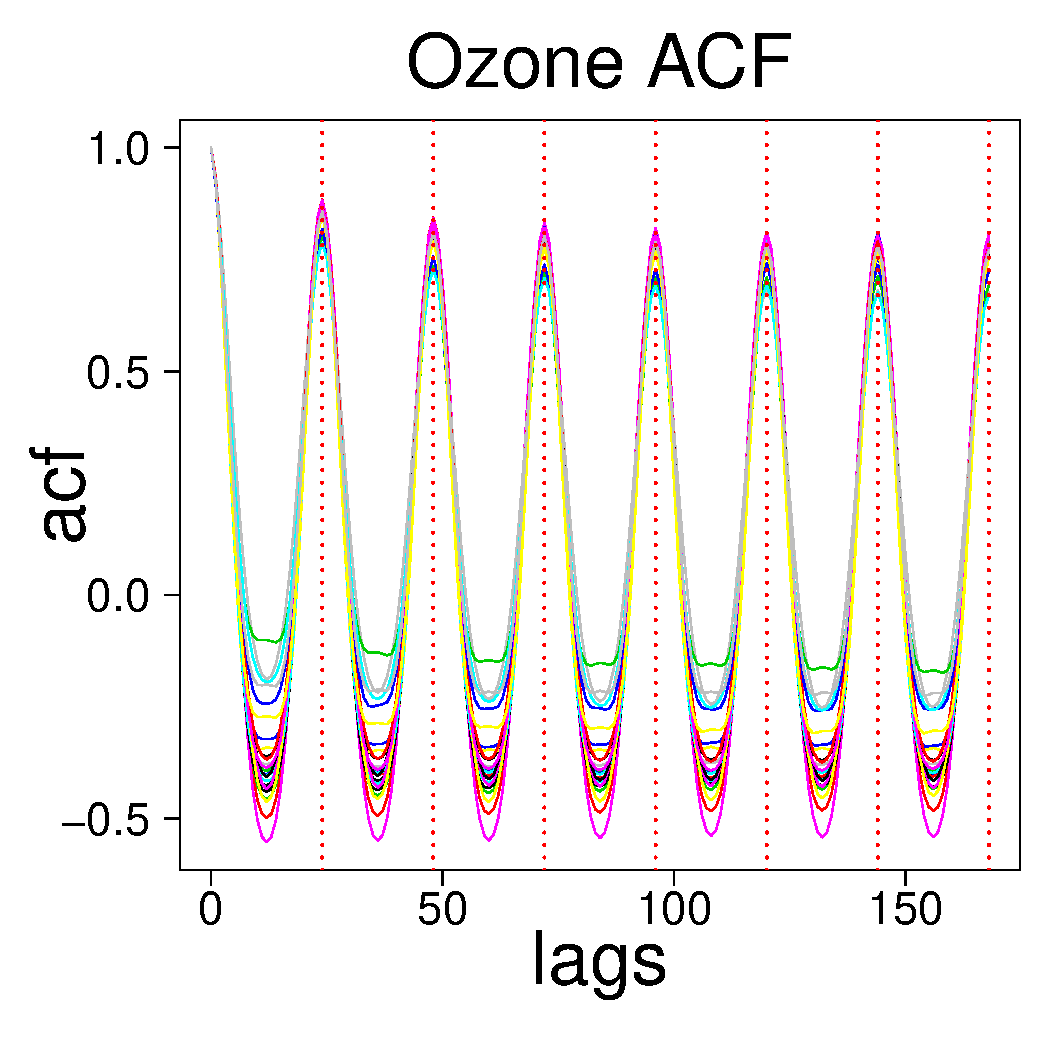
\includegraphics[width=\textwidth]{acf_o3.pdf}
      \subcaption{$\text{O}_{3}$ ACF}
   \end{subfigure}
  \begin{subfigure}[b]{.24\textwidth}
     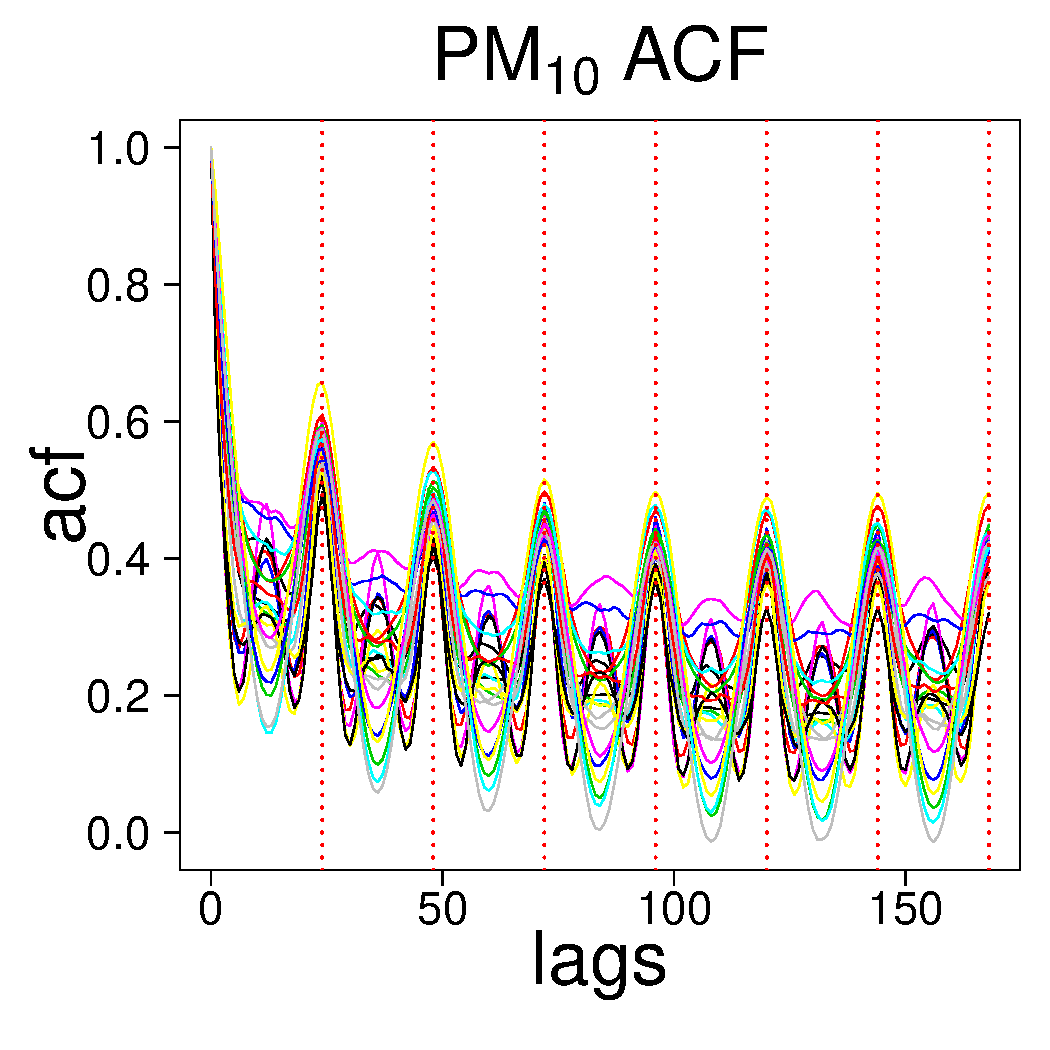
\includegraphics[width=\textwidth]{acf_pm10.pdf}
           \subcaption{$\text{PM}_{10}$  ACF}
   \end{subfigure}
    \begin{subfigure}[b]{.24\textwidth}
     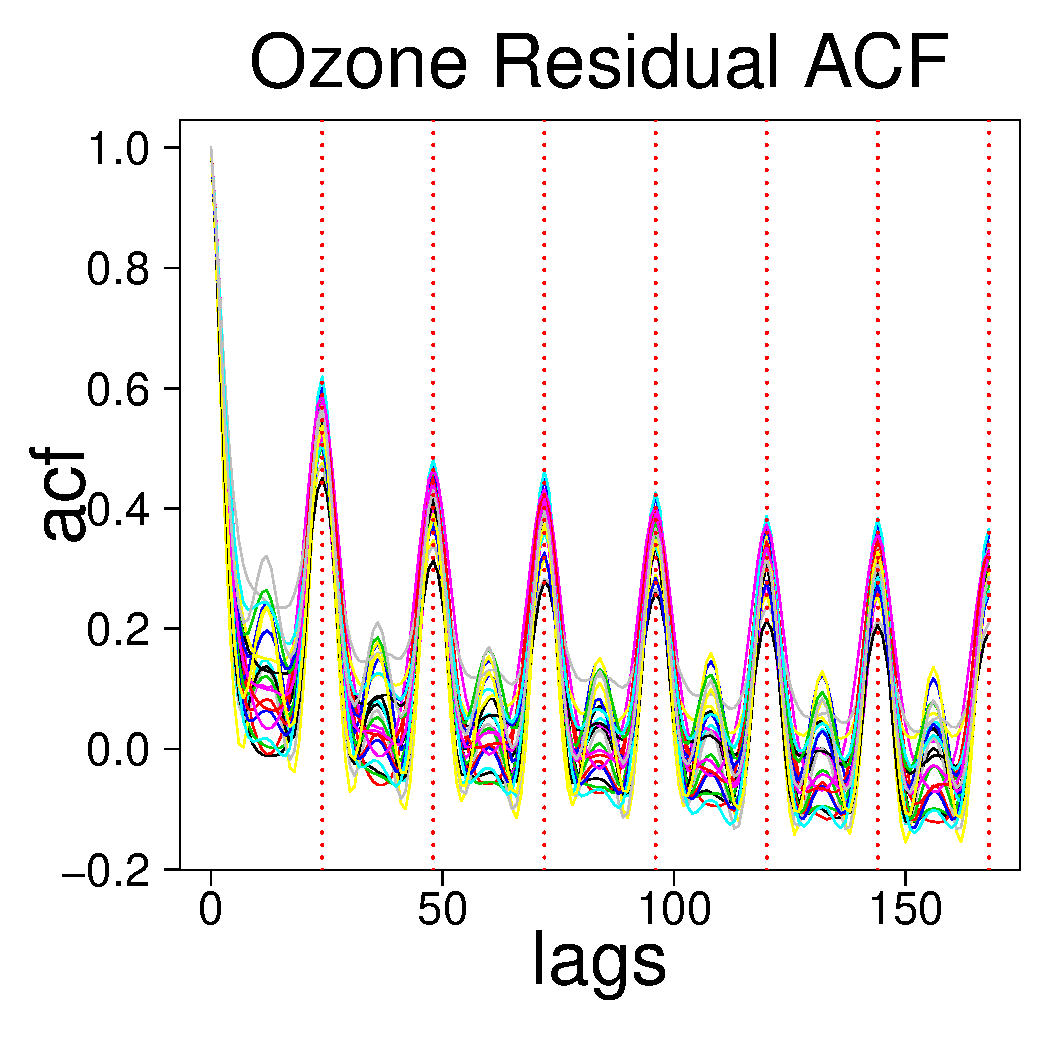
\includegraphics[width=\textwidth]{acf_o3_res.pdf}
           \subcaption{$\text{O}_{3}$ residual ACF}
   \end{subfigure}
     \begin{subfigure}[b]{.24\textwidth}
     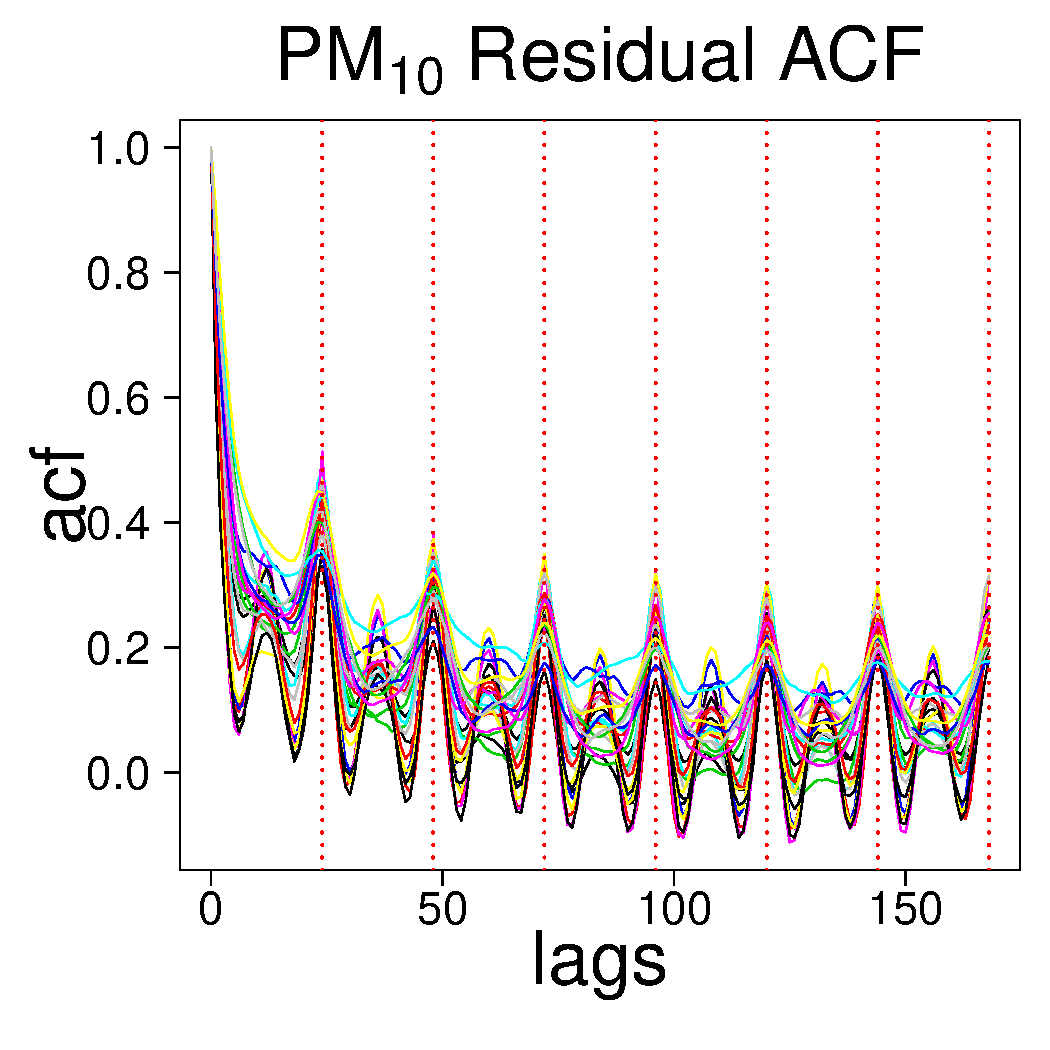
\includegraphics[width=\textwidth]{acf_pm10_res.pdf}
           \subcaption{$\text{PM}_{10}$  residual ACF}
   \end{subfigure}
  \end{center}
  \vspace{-4mm}
       \caption{Site-specific autocorrelation functions for ozone and $\text{PM}_{10}$ for one week of lags. }\label{fig:acf}
\end{figure}
}
\vspace{-3mm}
We also examined partial ACF plots to gain insight into which autoregressive lags may be necessary in the model; however, we found them to be uninformative given the strong seasonality of the data. Ultimately, we use out-of-sample predictive performance to select the autoregressive structure for ozone and $\text{PM}_{10}$.

We plot site-specific means for both pollutants in two ways.  We consider hourly means (Figures \ref{fig:hour_mean_ozone} and \ref{fig:hour_mean_pm10}), aggregated over the year, and daily means over the course of the year (Figures \ref{fig:day_mean_ozone} and \ref{fig:day_mean_pm10}). Figure \ref{fig:hour_mean_ozone} show that ozone concentrations generally peak around 4 pm (the warmest time of the day). In general, the highest ozone levels in Mexico City occur during spring months and June. In 2017, May, June, and July have the highest average ozone levels (see Figure \ref{fig:day_mean_ozone}). Figure \ref{fig:hour_mean_pm10} shows two daily peaks in $\text{PM}_{10}$ concentrations corresponding to commuting hours; however, annual trends for $\text{PM}_{10}$ are less clear in Figure \ref{fig:day_mean_pm10}.
We also plot standard deviation of ozone and $\text{PM}_{10}$ concentrations as a function of hour of the day for all stations in Figures \ref{fig:hour_sd_ozone} and \ref{fig:hour_sd_pm10}. Note that there is strong correlation between the standard deviation and the mean for both pollutants (compare Figures \ref{fig:hour_mean_ozone} and \ref{fig:hour_sd_ozone} and compare Figures \ref{fig:hour_mean_pm10} and \ref{fig:hour_sd_pm10}). This correlation could be addressed through modeling in a variety of ways. First, and most simply, one could use a variance stabilizing transformation (VST) to address the correlation between the mean and variance (e.g. log, square-root, Box-Cox). Alternatively, we could use heteroscedastic models that specify variance directly as a function of hour or month.
\vspace{-3mm}
\begin{figure}[H]
  \begin{center}
   \begin{subfigure}[b]{.3\textwidth}
      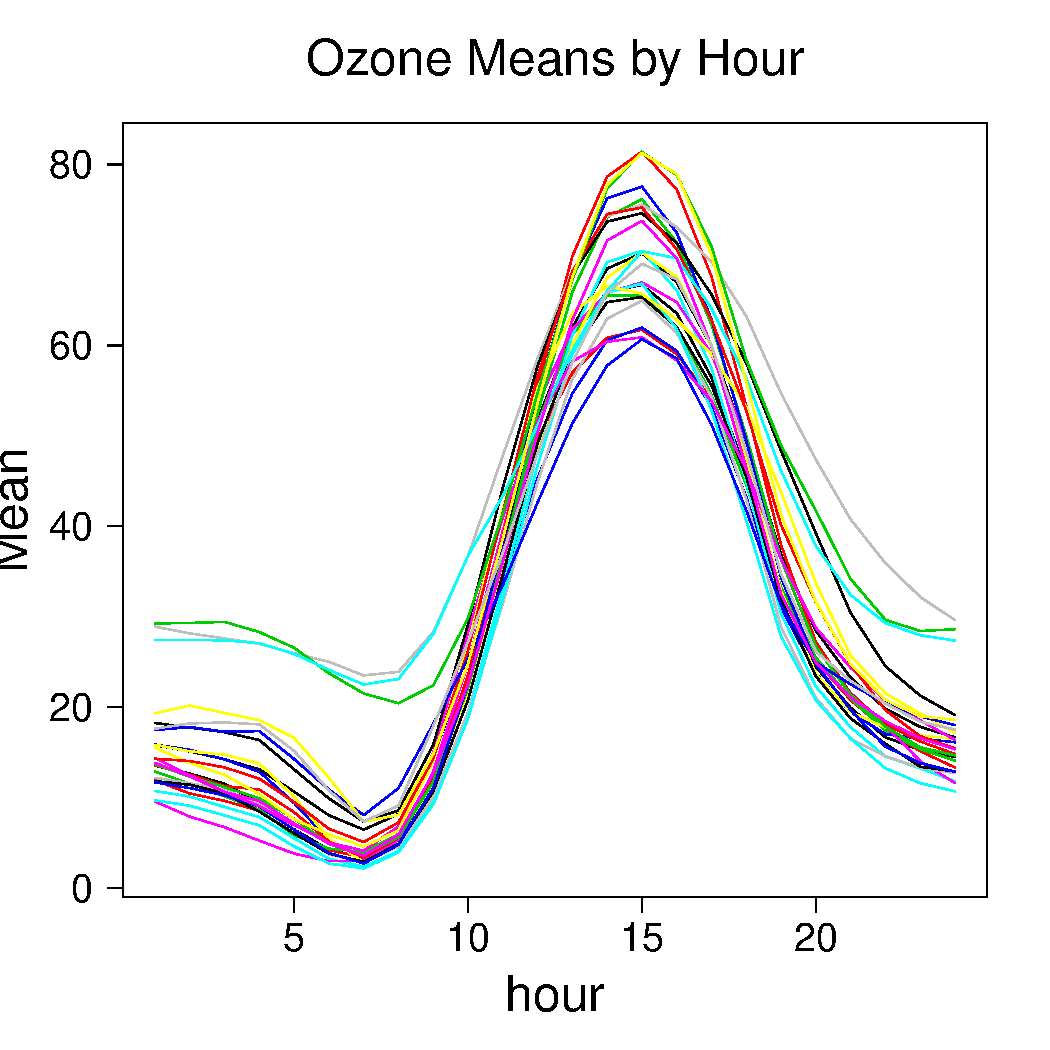
\includegraphics[width=\textwidth]{hour_mean_O3.pdf}
      \subcaption{Hourly ozone means}\label{fig:hour_mean_ozone}
   \end{subfigure}
              \begin{subfigure}[b]{.3\textwidth}
      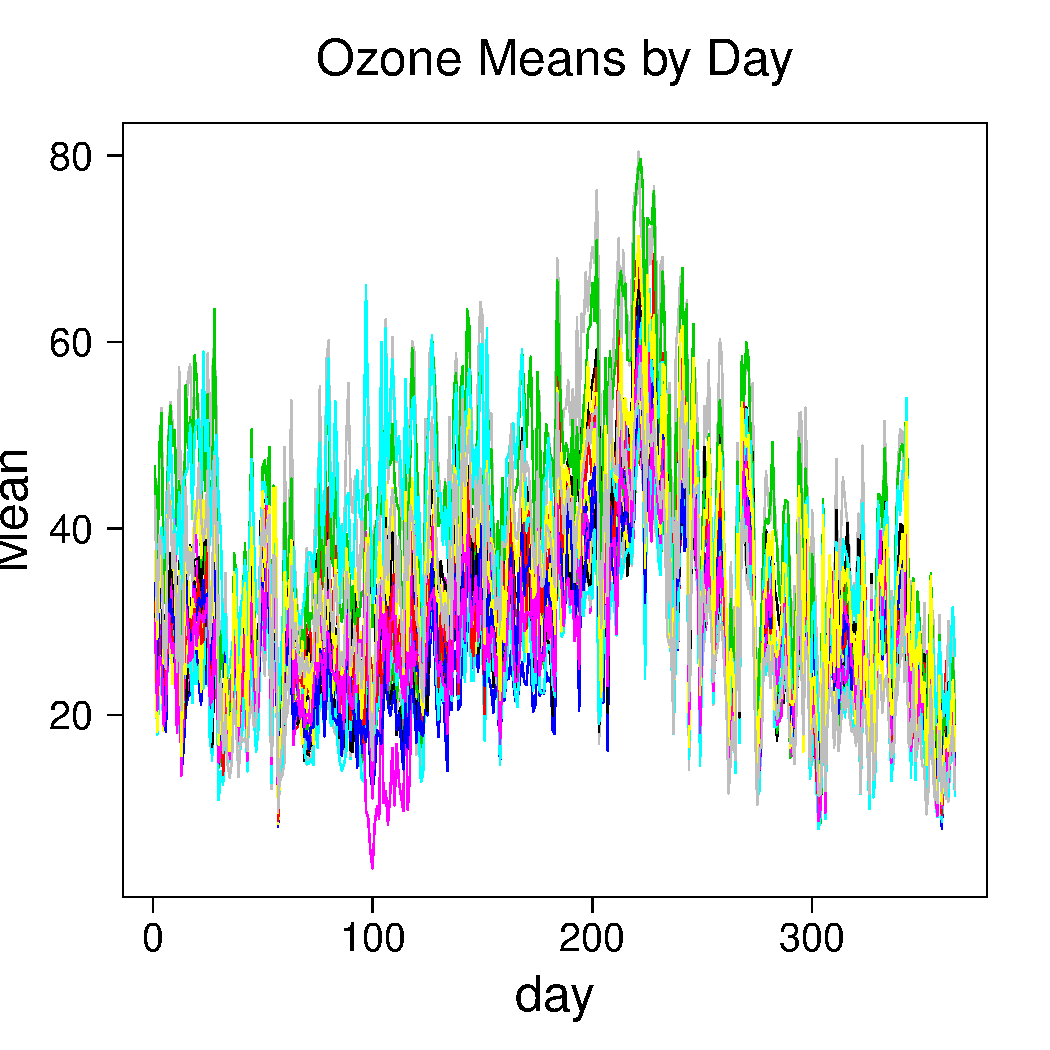
\includegraphics[width=\textwidth]{day_mean_O3}
            \subcaption{Daily ozone means}\label{fig:day_mean_ozone}
         \end{subfigure}
      \begin{subfigure}[b]{.3\textwidth}
      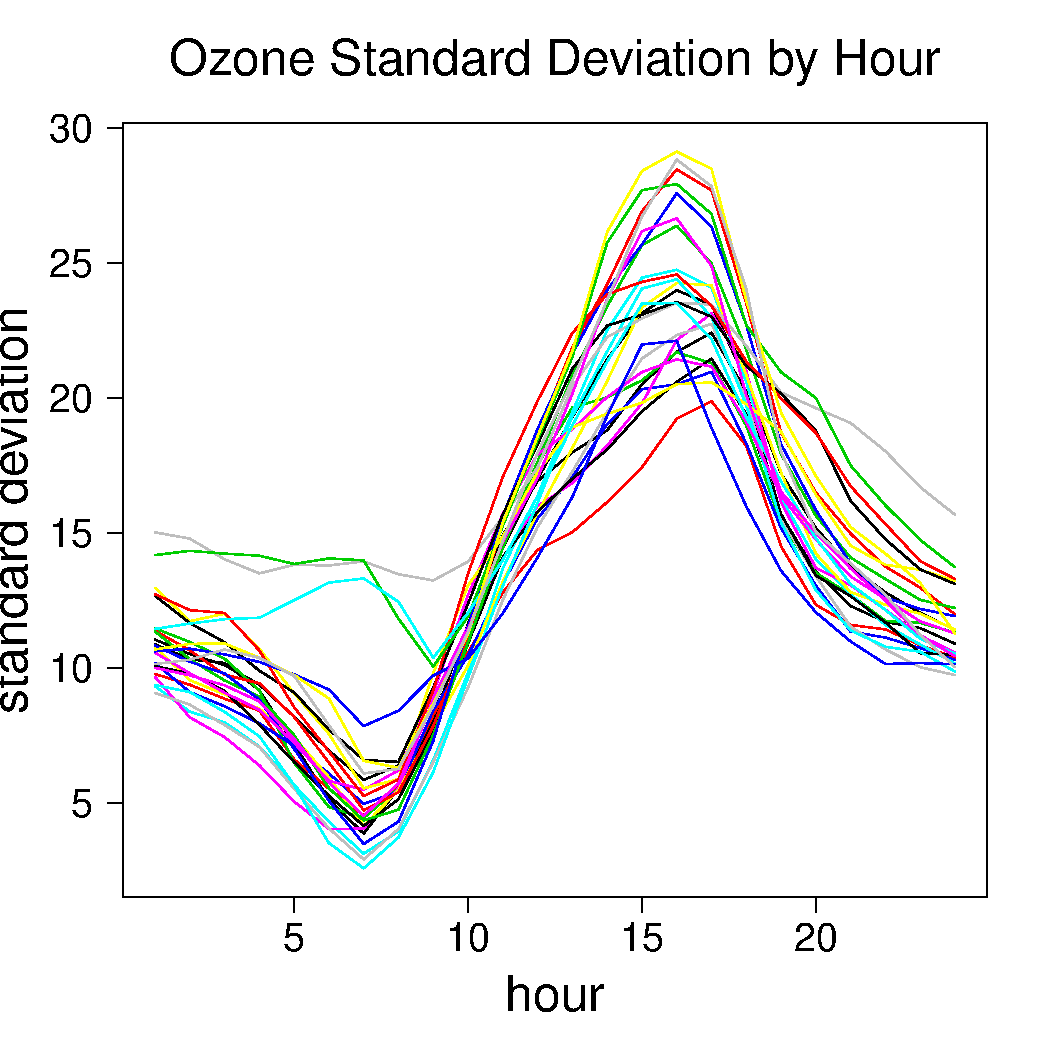
\includegraphics[width=\textwidth]{hour_sd_O3.pdf}
      \subcaption{Hourly ozone std. dev.}\label{fig:hour_sd_ozone}
   \end{subfigure}
  \end{center}
  \vspace{-5mm}
       \caption{Site-specific means by hour averaged over the year}\label{fig:hour_mean}
\end{figure}
\vspace{-5mm}
\begin{figure}[H]
  \begin{center}
    \begin{subfigure}[b]{.3\textwidth}
      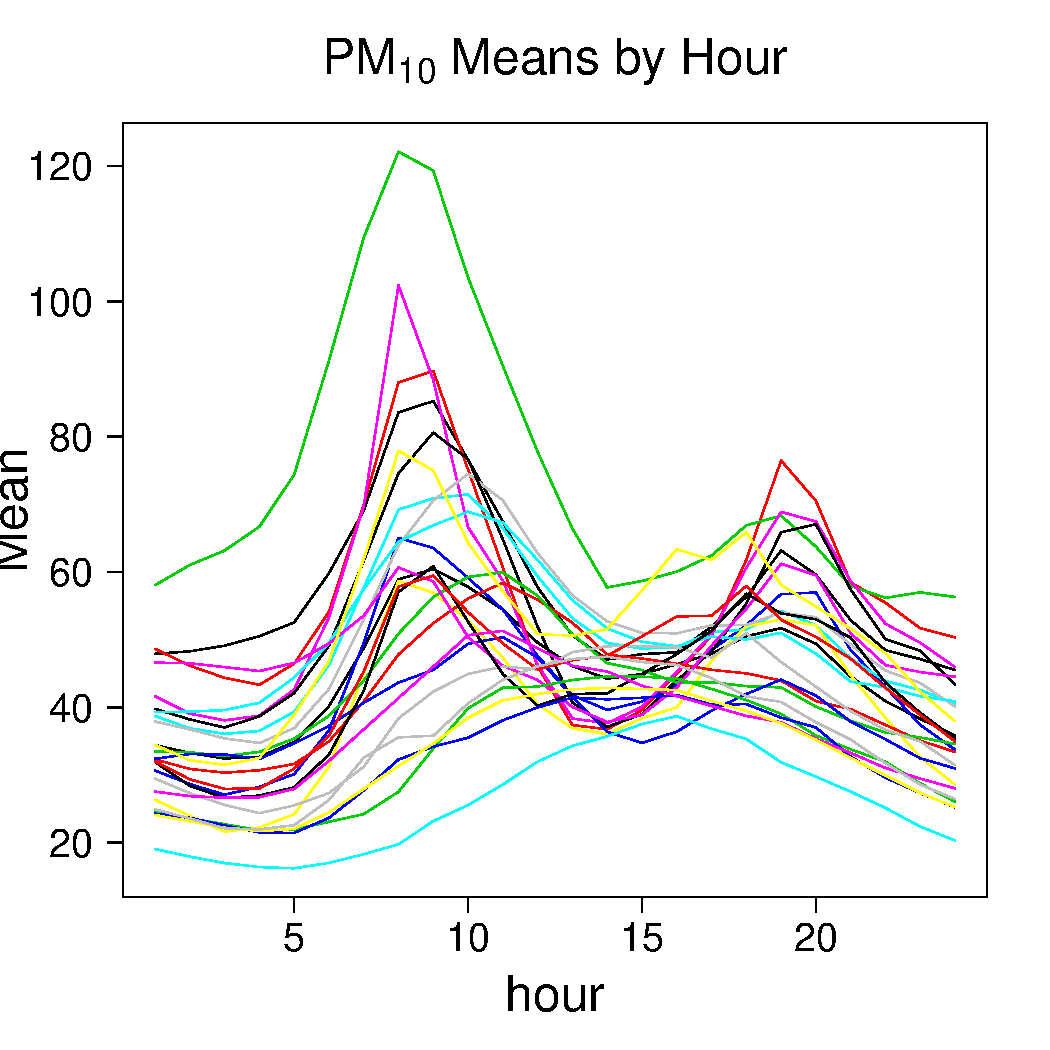
\includegraphics[width=\textwidth]{hour_mean_PM10}
            \subcaption{Hourly $\text{PM}_{10}$ means}\label{fig:hour_mean_pm10}
         \end{subfigure}
                    \begin{subfigure}[b]{.3\textwidth}
      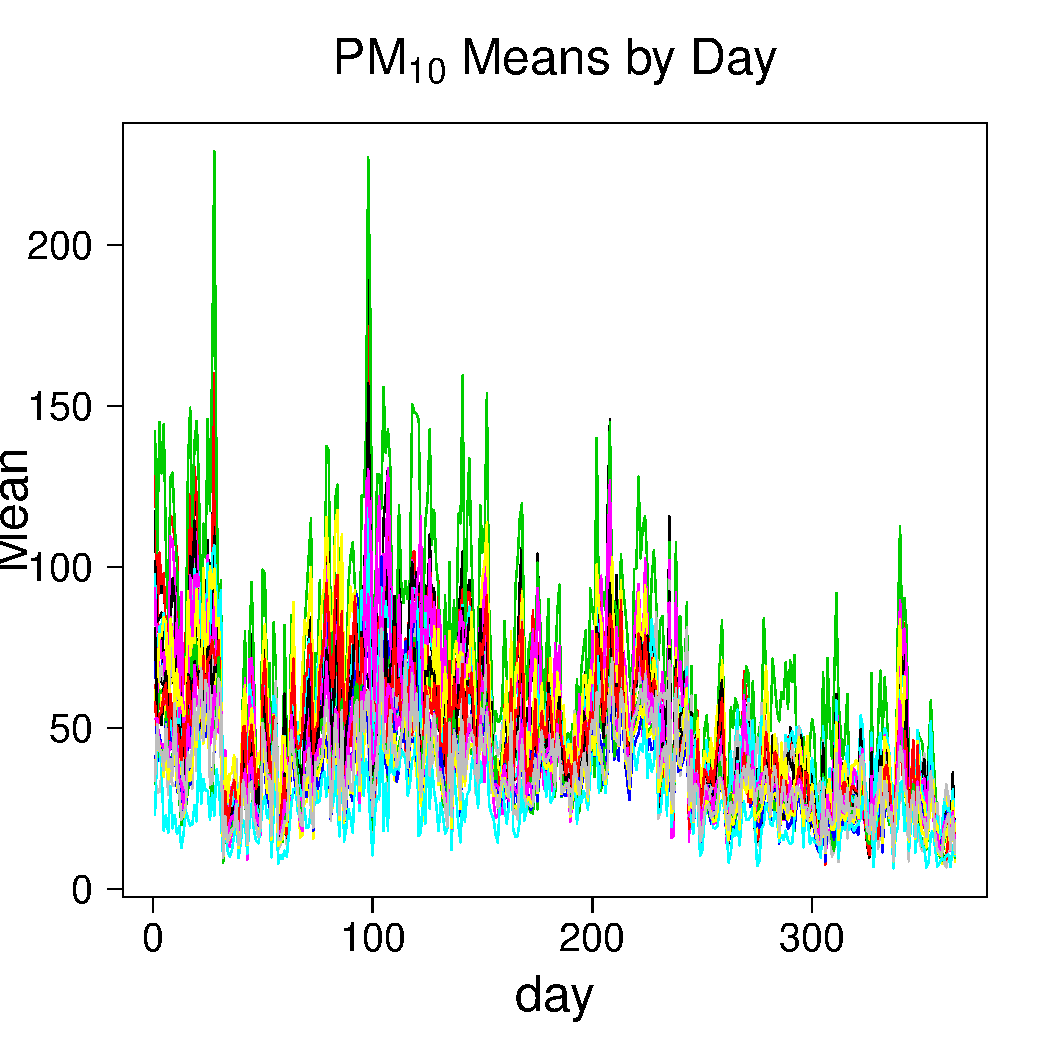
\includegraphics[width=\textwidth]{day_mean_PM10.pdf}
            \subcaption{Daily $\text{PM}_{10}$ means}\label{fig:day_mean_pm10}
         \end{subfigure}
           \begin{subfigure}[b]{.3\textwidth}
      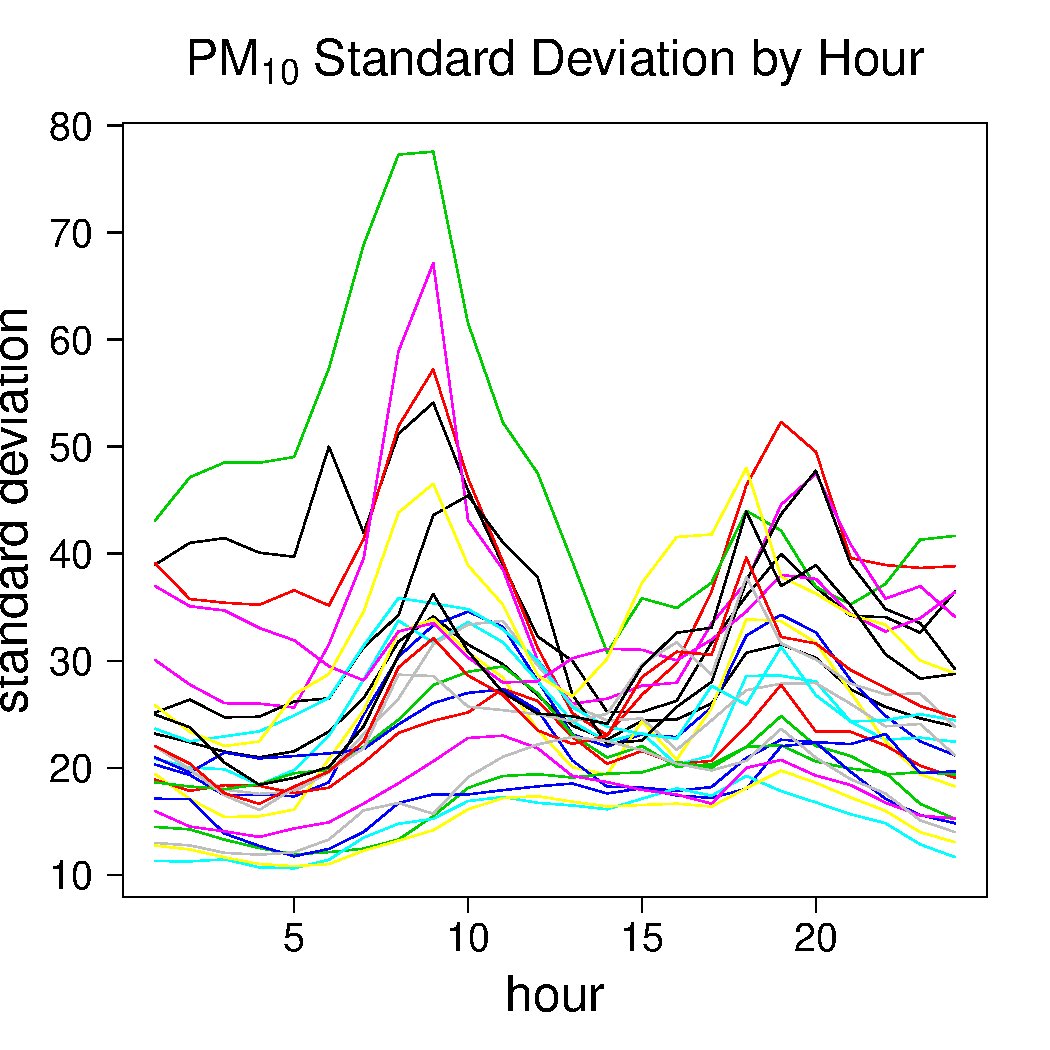
\includegraphics[width=\textwidth]{hour_sd_PM10}
            \subcaption{Hourly $\text{PM}_{10}$ std. dev.}\label{fig:hour_sd_pm10}
         \end{subfigure}
  \end{center}
  \vspace{-5mm}
       \caption{Site-specific  hourly means, means averaged over every day, and standard deviations over hour of the day}\label{fig:pm10}
\end{figure}
\vspace{-5mm}

To further investigate the relationship between the mean and variance, we fit a simple AR model with site-specific regression and AR coefficients and explore the residuals as a function of the mean. We include lags 1, 2, 24, and 168. After fitting the model, we bin observations according to their mean and calculate the variance of the associated residuals within that bin. The results for ozone and $\text{PM}_{10}$ concentration are in Figure \ref{fig:mean_var}. These plots suggest that using VST's may effectively address the correlation between the mean and variance of model residuals. Specifically, the mean-variance relationship for ozone is strong (and approximately linear for values less than 50 ppb), and the mean-variance relationship for $\text{PM}_{10}$ appears to be approximately quadratic. Linear mean-variance relationships are stabilized by a square-root transformation, and quadratic mean-variance associations are roughly removed using log transformations \citep[see, for example, Section 3.3. in][]{hocking2013}.
\vspace{-3mm}
\begin{figure}[H]
  \begin{center}
   \begin{subfigure}[b]{.45\textwidth}
      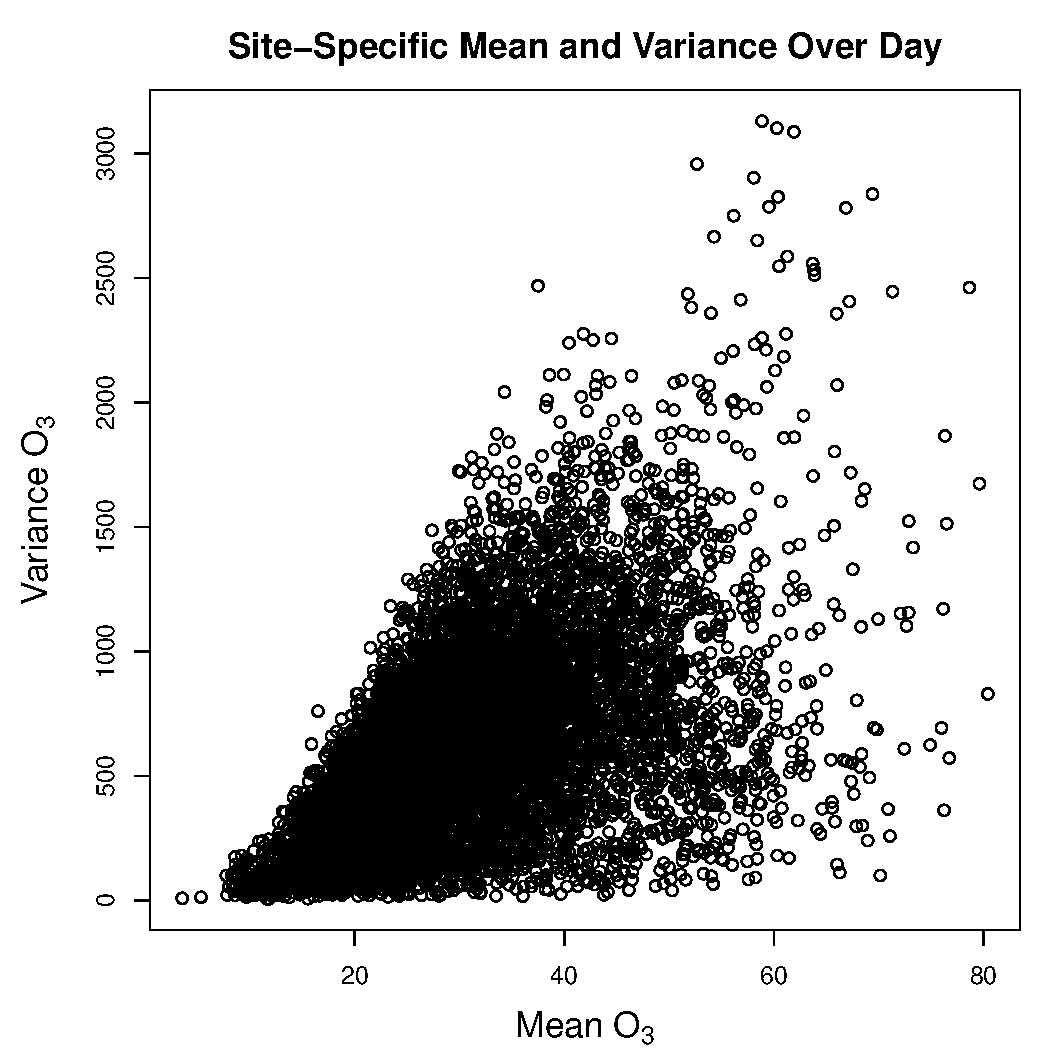
\includegraphics[width=.9\textwidth]{ozone_mean_var}
      \subcaption{$\text{O}_{3}$ mean-variance}
   \end{subfigure}
   \hspace{10mm}
     \begin{subfigure}[b]{.45\textwidth}
     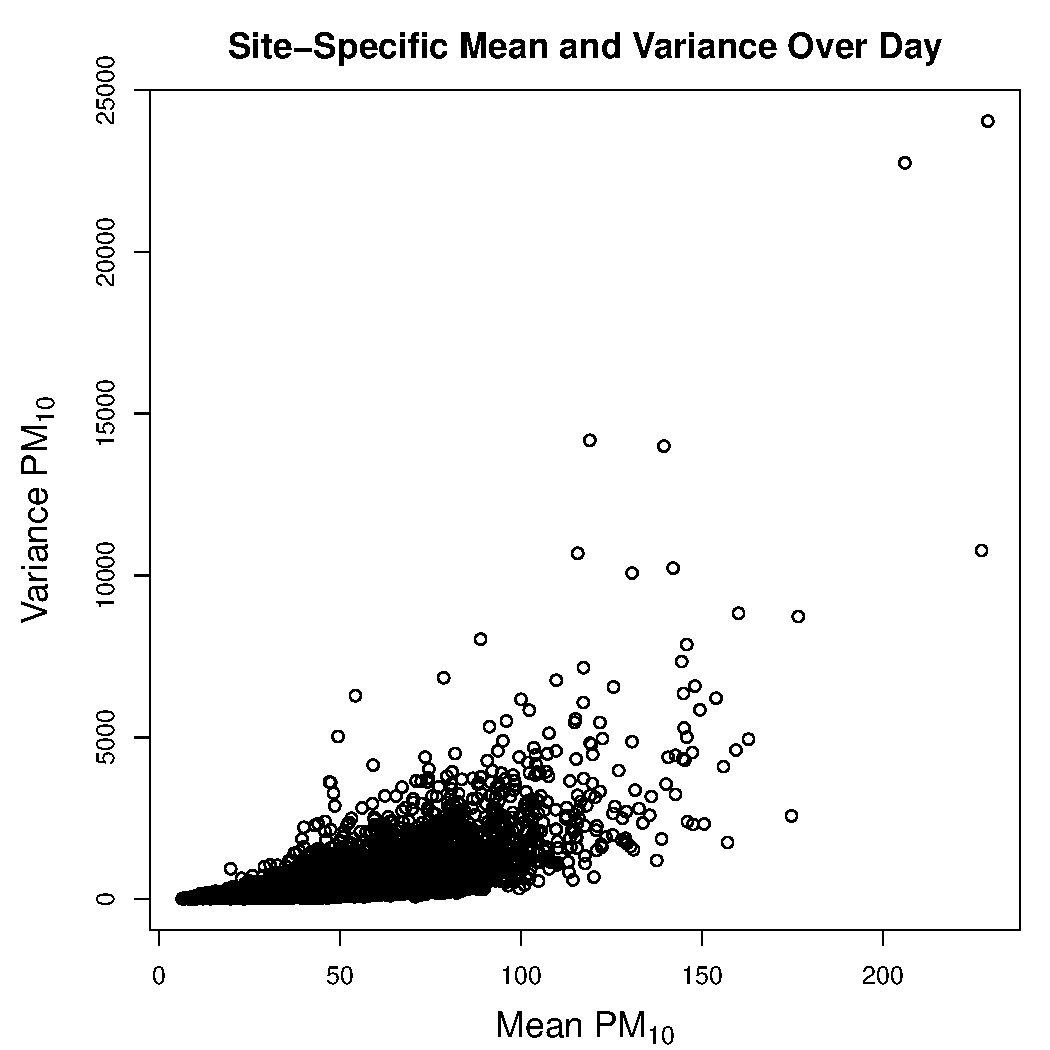
\includegraphics[width=.9\textwidth]{pm10_mean_var}
           \subcaption{$\text{PM}_{10}$ mean-variance}
   \end{subfigure}
  \end{center}
  \vspace{-4mm}
       \caption{Binned residual variance for ozone and $\text{PM}_{10}$ plotted against mean.}\label{fig:mean_var}
\end{figure}

\section{Model Selection and Prediction of Held-out Data}\label{app:full_cond_pred}

This model selection centers around how many and which lagged terms should be used in our spatiotemporal model. For model comparison, we hold out 10\% of the data and impute or update these held-out values each step of the Gibbs sampler which is described below.
\begin{align*}
\mu_{1it} &= \bx_{i(t-1)}^T \bbeta_{1i} + {\bL^{O}_{it}}^T\bgamma_{1i}+ \psi_{1i}, \\
\mu_{2it} &= \bx_{i(t-1)}^T \bbeta_{2i} + {\bL^{PM}_{it}}^T\bgamma_{2i}+ \psi_{2i},
\end{align*}
and let $Y^{O}_{it} | \cdots$ and $Y^{PM}_{it} | \cdots$ denote the full conditional distributions of missing observations. For the heteroscedastic model, the full conditional distributions for the missing data are
\begin{align*}
Y^{O}_{it} | \cdots &\sim N( \tau^*_{1it} \mu^*_{1it},\tau^*_{1it} ) \\
Y^{PM}_{it} | \cdots &\sim N( \tau^*_{2it} \mu^*_{2it},\tau^*_{2it} ) \nonumber
\end{align*}
with
\begin{align*}
\tau^*_{1it} &=  \left(\frac{1}{\sigma^2_{1t} } + \sum^{n_{1l}}_{j=1} \frac{\gamma_{1j}^2}{\sigma^2_{1(t+ l_{1j})}} \right)^{-1} \\
\mu^*_{1it} &= \mu_{1it} + \sum_{j=1}^{n_{ 1l } } \frac{ \gamma_{1ij} ( Y^{O}_{i(t + l_{1j} )} - m_{1i(t + l_{1j})} + \gamma_{1ij}  Y^{O}_{it} )}{ \sigma^2_{1(t+l_{1j})} }  \\
\tau^*_{2it} &= \left(\frac{1}{\sigma^2_{2t} } + \sum^{n_{2l}}_{j=1} \frac{\gamma_{2j}^2}{\sigma^2_{2(t+ l_{2j})}} \right)^{-1} \\
\mu^*_{2it} &= \mu_{2it} + \sum_{j=1}^{n_{ 2l } } \frac{ \gamma_{2ij} ( Y^{PM}_{i(t + l_{2j} )} - m_{2i(t + l_{2j} )} + \gamma_{2ij} Y^{PM}_{it} )}{ \sigma^2_{2(t+l_{2j} )} },
\end{align*}
where $l_{1j}$ is the $j^\text{th}$ lag for ozone with coefficient $\gamma_{1ij}$ and $l_{2j}$ is the $j^\text{th}$ lag for $\text{PM}_{10}$  with coefficient $\gamma_{1ij}$. The imputation method for the homoscedastic model is a special case of the heteroscedastic model.

The heteroscedastic models with variance that varies over hour of the day and month of the year performed uniformly worse than homoscedastic counterparts that used VST's (results not shown). Examining various combinations of square-root transformations, log transformations, and truncated distributions, we found that models using the square-root transformation for ozone and the log transformation for $\text{PM}_{10}$ gave the best predictive performance. So, for model selection, we only provide the results for six models which use the square-root transformation for ozone and the log-transformation for $\text{PM}_{10}$ but differ in terms of the lagged terms are included in the model. The results of this comparison are given in Table \ref{tab:mod_comp}.

We further note that in preliminary model comparison, we found that models which included a lag-3 and other higher order lags or that excluded lag-2 saw no improvement in terms of prediction; thus, we arrived at the models included in Table \ref{tab:mod_comp}. Given these results, though the differences are modest, we adopt the model for ozone and $\text{PM}_{10}$ uses lags 1, 2, 24, and 168 and the ensuing results are presented for this model.

Turning to which terms of our spatiotemporal model are used. We address whether ozone and $\text{PM}_{10}$ random effects should be modeled jointly or whether they should be included in the model altogether. To do this, we compare out-of-sample predictive performance of various reduced models to the full model where spatial random effects for ozone and $\text{PM}_{10}$ are modeled jointly. The performance of these models is presented in Table \ref{tab:mod_comp2}. The table reveals essentially no differences among the models, particularly allowing for Monte Carlo error in the values for the criteria. However, since the dependence spatial model is always preferred to the independence spatial model and since the dependence coefficient, $a_{12}^{(\phi)}$ is significantly positive (see Section \ref{sec:post_sum} below), we present results for the former in the manuscript.

\vspace{-3mm}
\begin{table}[H]
%\begin{longtable}{rrrrrrrrrrrr}
\centering
\scriptsize
\begin{tabular}{lllrrrrrrrrrr}
 & &  &  &  &  &  &  &  & & \\
 \hline
 & &   & $O_3$ & $O_3$  & $O_3$ & $O_3$ & $\text{PM}_{10}$ & $\text{PM}_{10}$  & $\text{PM}_{10}$ & $\text{PM}_{10}$ \\
  & Lags & ES & CRPS & RMSE  & MAE & Cov & CRPS & RMSE  & MAE & Cov \\
  \hline
%1 & TN  & (1,2) & 2.58 & 5.00 & 3.34 & 0.90 & 6.90 & 14.21 & 8.58 & 0.93 \\
%2 & TN  & (1,24) & 3.10 & 5.61 & 3.88 & 0.96 & 6.85 & 14.05 & 8.55 & 0.93 \\
%3 & TN & (1,2,24) & 2.57 & 4.96 & 3.34 & 0.90 & 6.85 & 14.03 & 8.54 & 0.93 \\
%4 & TN  & (1,2,12,24) & 2.57 & 4.97 & 3.35 & 0.90 & 6.86 & 14.05 & 8.56 & 0.93 \\
%5 & TN & (1:24) & 2.56 & 4.92 & 3.32 & 0.91 & 6.79 & 13.90 & 8.47 & 0.93 \\
%6 & TN & (1,24,168) & 3.08 & 5.57 & 3.86 & 0.96 & 6.85 & 14.02 & 8.55 & 0.93 \\
%7 & TN & (1,2,24,168) & 2.56 & 4.94 & 3.33 & 0.90 & 6.84 & 14.01 & 8.54 &  0.93 \\
%8 & TN& (1,2,12,24,168) & 2.57 & 4.95 & 3.34 & 0.90 & 6.85 & 14.01 & 8.56 & 0.93 \\
%9 & TN & (1:24,168) & 2.58 & 4.95 & 3.35 & 0.91 & 6.78 & 13.88 & 8.47 & 0.93 \\
%%%%%%%%%%%%%%%%%%%%%%%%%%%%%%%%%%
%9 & LN  & (1,2) & 3.48 & 5.81 & 3.88 & 0.90 & 6.68 & 14.52 & 8.72 & 0.92 \\
%10 & LN  & (1,24) & 3.85 & 5.66 & 3.91 & 0.94 & 6.57 & 14.12 & 8.58 & 0.92 \\
%11 & LN  & (1,2,24) & 3.35 & 5.39 & 3.63 & 0.91 & 6.57 & 14.13 & 8.58 & 0.92 \\
%12 & LN  & (1,2,12,24) & 3.36 & 5.51 & 3.73 & 0.91 & 6.56 & 14.10 & 8.62 & 0.92 \\
%13 & LN  & (1:24) & 3.33 & 5.46 & 3.72 & 0.91 & 6.50 & 13.95 & 8.49 & 0.92 \\
%14 & LN & (1,24,168) & 3.80 & 5.61 & 3.88 & 0.94 & 6.54 & 14.06 & 8.55 & 0.92 \\
%15 & LN & (1,2,24,168) & 3.35 & 5.36 & 3.62 & 0.91 & 6.55 & 14.08 & 8.60 &  0.92 \\
%16 & LN& (1,2,12,24,168) & 3.35 & 5.34 & 3.61 & 0.91 & 6.55 & 14.08 & 8.60 & 0.92 \\
%18 & LN & (1:24,168) & 3.36 & 5.63 & 3.83 & 0.91 & 6.49 & 13.91 & 8.50 & 0.92 \\
%%%%%%%%%%%%%%%%%%%%%%%%%%%%%%%%%%%
1 &  (1,2) & 0.2552 & 2.5392 & 5.0448 & 3.3409 & 0.8867 & 6.7263 & 14.5427 & 8.7725 & 0.9228 \\
2  & (1,2,24)& 0.2513 & 2.5158 & 4.9709 & 3.3035 & 0.8925 & 6.6176 & 14.1469 & 8.6189 & \textbf{0.9217} \\
\textbf{3}  & (1,2,24,168)&\textbf{0.2505} & \textbf{2.5140} & \textbf{4.9614} & \textbf{3.2982} & \textbf{0.8941} & \textbf{6.5947} & \textbf{14.0922} & \textbf{8.6285} &  0.9229 \\
4 &  (1,2,12) & 0.2540 & 2.5298 & 5.0274 & 3.3244 & 0.8887 & 6.6959 & 14.4314 & 8.7864 & 0.9230 \\
5  & (1,2,12,24)& 0.2509 & 2.5168 & 4.9726 & 3.3115 & 0.8917 & 6.6035 & 14.0981 & 8.6296 & 0.9220 \\
6  & (1,2,12,24,168)& 0.2507 & 2.5154 & 4.9651 & 3.2993 & \textbf{0.8941} & 6.5976 & 14.0972 & 8.6378 &  0.9225 \\
%7 & (1:24)& 0.2502 & 2.5214 & 4.9608 & 3.3202 & 0.8995 & 6.5780 & 14.0103 & 8.5623 & 0.9244 \\
%8  & (1:24,168)& 0.25 & 2.58 & 5.08 & 3.39 & 0.91 & 6.49 & 13.91 & 8.50 & 0.92 \\
%%%%%%%%%%%%%%%%%%%%%%%%%%%%%%%%%%
%1 & TN & H & (1,2) & 2.95 & 5.03 & 3.38 & 0.98 & 7.49 & 15.21 & 9.58 & 0.94 \\
%2 & TN & H & (1,24) & 3.19 & 5.61 & 3.87 & 0.98 & 7.65 & 15.39 & 9.96 & 0.93 \\
%3 & TN& H & (1,2,24) & 2.91 & 5.04 & 3.41 & 0.97 & 8.52 & 16.93 & 11.14 & 0.90 \\
%4 & TN & H & (1,2,12,24) & 2.92 & 5.05 & 3.44 & 0.98 & 10.98 & 23.17 & 14.66 & 0.87 \\
%5 & TN& H & (1:24) & 2.85 & 5.03 & 3.42 & 0.97 & 7.67 & 15.30 & 10.02 & 0.93 \\
%6 & TN& H & (1,24,168) & 3.16 & 5.57 & 3.86 & 0.98 & 8.29 & 16.55 & 10.85 & 0.91 \\
%7 & TN& H & (1,2,24,168) & 2.91 & 5.03 & 3.43 & 0.98 & 13.08 & 32.45 & 16.53 &  0.89 \\
%8 & TN& H& (1,2,12,24,168) & 2.90 & 5.02 & 3.41 & 0.98 & 9.67 & 19.23 & 12.99 & 0.88 \\
%9 & TN& H & (1:24,168) & 2.86 & 5.06 & 3.47 & 0.97 & 10.34 & 52.78 & 20.21 & 0.89 \\
%%%%%%%%%%%%%%%%%%%%%%%%%%%%%%%%%%%
%28 & LN & H & (1,2) & 3.61 & 5.86 & 3.98 & 0.96 & 8.11 & 17.95 & 11.49 & 0.91 \\
%29 & LN & H & (1,24) & 3.66 & 5.91 & 4.12 & 0.97 & 7.82 & 17.20 & 11.12 & 0.91 \\
%30 & LN& H & (1,2,24) & 3.52 & 5.64 & 3.86 & 0.96 & 7.95 & 17.35 & 11.51 & 0.91 \\
%31 & LN & H & (1,2,12,24) & 3.50 & 5.78 & 4.01 & 0.96 & 7.03 & 14.90 & 9.24 & 0.93 \\
%32 & LN& H & (1:24) & 3.36 & 5.53 & 3.83 & 0.96 & 6.92 & 14.81 & 9.14 & 0.93 \\
%33 & LN& H & (1,24,168) & 3.65 & 5.96 & 4.15 & 0.97 & 7.89 & 17.47 & 11.33 & 0.91 \\
%34 & LN& H & (1,2,24,168) & 3.50 & 5.71 & 3.92 & 0.96 & 7.36 & 15.76 & 10.10 &  0.92 \\
%35 & LN& H& (1,2,12,24,168) & 3.48 & 5.62 & 3.86 & 0.96 & 7.85 & 17.31 & 11.14 & 0.91 \\
%36 & LN& H & (1:24,168) & - & - & - & - & - & - & - & - \\
   \hline
\end{tabular}
\caption{Predictive model comparison. The ``Lags'' label indicates which lags are used for both outcomes. ``ES,'' ``CRPS,'' ``MSE,'' ``MAE,'' and ``Cov'' head columns giving ES, CRPS, MSE, MAE, and 90\% prediction interval coverage. Best performances are indicated with bold text.
%\textbf{Models with dashes haven't finished running, except 36. This model had major stability issues. These models are really slow with missing data because the lags change with imputation, so this doesn't scale super well. }
}\label{tab:mod_comp}
\end{table}

\vspace{-3mm}
\begin{table}[H]
%\begin{longtable}{rrrrrrrrrrrr}
\centering
\scriptsize
\begin{tabular}{lllrrrrrrrrrr}
 & &  &  &  &  &  &  &  & & \\
 \hline
 & &   & $O_3$ & $O_3$  & $O_3$ & $O_3$ & $\text{PM}_{10}$ & $\text{PM}_{10}$  & $\text{PM}_{10}$ & $\text{PM}_{10}$ \\
  & Model Constraints & ES & CRPS & RMSE  & MAE & Cov & CRPS & RMSE  & MAE & Cov \\
  \hline
1 & $\bV_1 = 0$  & 0.2507 & 2.5141 & 4.9622 & 3.2982 & 0.8938 & 6.5986 & 14.1055 & 8.6298 & 0.9225  \\
2 & $\bV_2 = 0$   & 0.2505 & 2.5150 & 4.9637 & 3.2986 & 0.8936 & 6.5915 & 14.0853 & 8.6135 & 0.9229  \\
3 & $\bV_1 = \bV_2 = 0$  & 0.2505 & 2.5149 & 4.9635 & 3.2991 & 0.8941 & 6.5897 & 14.0837 & 8.6085 & 0.9234  \\
4 & $a_{12}^{(\psi)} = 0$ & 0.2509 & 2.5156 & 4.9635 & 3.3004 & 0.8941 & 6.6032 & 14.1193 & 8.6447 & 0.9237  \\
5  & Full Model & 0.2505 & 2.5140 & 4.9614 & 3.2982 & 0.8941 & 6.5947 & 14.0922 & 8.6285 &  0.9229 \\
% & w = exp(- 3d$\times$ max)1,2,24,168) &  0.2505 & 2.5140 & 4.9613 & 3.2982 & 0.8941 & 6.5934 & 14.0866 & 8.6280 & 0.9230  \\
%& w = exp(- 10d$\times$ max) & 0.2504 & 2.5146 & 4.9618 & 3.2991 & 0.8943 & 6.5897 & 14.0716 & 8.6296 & 0.9229  \\
%& w = exp(- 1/10d$\times$ max) &  0.2506 & 2.5140 & 4.9615 & 3.2982 & 0.8941 & 6.5950 & 14.0935 & 8.6285 & 0.9229  \\
%& w = exp(- 1/3d$\times$ max) &  0.2506 & 2.5140 & 4.9615 & 3.2982 %& 0.8941 & 6.5949 & 14.0932 & 8.6285 & 0.9229  \\
   \hline
\end{tabular}
\caption{Predictive model comparison. The ``Lags'' label indicates which lags are used for both outcomes. ``ES,'' ``CRPS,'' ``MSE,'' ``MAE,'' and ``Cov'' head columns giving ES, CRPS, MSE, MAE, and 90\% prediction interval coverage. Best performances are indicated with bold text.
%\textbf{Models with dashes haven't finished running, except 36. This model had major stability issues. These models are really slow with missing data because the lags change with imputation, so this doesn't scale super well. }
}\label{tab:mod_comp2}
\end{table}


\section{Posterior Summaries and Discussion}\label{sec:post_sum}

Posterior summaries for covariance parameters ($\sigma^2_1$, $\sigma^2_2$, $a^{(\psi)}_{11}$, $a^{(\psi)}_{12}$, and $a^{(\psi)}_{22}$) and the overall means for hierarchical coefficient parameters ($\bbeta_{01}$,$\bbeta_{02}$,$\bgamma_{01}$,$\bgamma_{02}$) are given in Table \ref{tab:post_sum}.

\vspace{-2mm}
\begin{table}[H]
\centering
\footnotesize
\begin{tabular}{lrrrr}
  \hline
 & Mean & Std Dev & 2.5\% & 97.5\% \\
  \hline
\rule{0pt}{2.2ex}$\sigma^2_1$ & 0.5180 & 0.0016 & 0.5148 & 0.5211 \\
$\sigma^2_2$ & 0.1490 & 0.0005 & 0.1481 & 0.1499 \\
$a_{11}^{(\psi)}$ & 0.5102 & 0.0857 & 0.3633 & 0.6988 \\
$a_{22}^{(\psi)}$ & 0.5203 & 0.1093 & 0.3176 & 0.7438 \\
$a_{12}^{(\psi)}$ & 0.4723 & 0.2622 & 0.0224 & 1.0090 \\
$\bbeta_{01}$ (Intercept) & 0.4503 & 0.0087 & 0.4330 & 0.4668 \\
$\bbeta_{01}$ (RH)  & -0.0027 & 0.0002 & -0.0031 & -0.0024 \\
$\bbeta_{01}$ (TMP)  & 0.0138 & 0.0019 & 0.0100 & 0.0176 \\
$\bbeta_{02}$ (Intercept) & 0.3573 & 0.0124 & 0.3300 & 0.3836 \\
$\bbeta_{02}$ (RH) & -0.0022 & 0.0002 & -0.0026 & -0.0018 \\
$\bbeta_{02}$ (TMP)  & -0.0093 & 0.0009 & -0.0110 & -0.0076 \\
$\bgamma_{01}$ (lag 1) & 1.0649 & 0.0113 & 1.0432 & 1.0878 \\
$\bgamma_{01}$ (lag 2) & -0.4079 & 0.0080 & -0.4238 & -0.3921 \\
$\bgamma_{01}$ (lag 24)  & 0.1683 & 0.0041 & 0.1603 & 0.1763 \\
$\bgamma_{01}$ (lag 168) & 0.0835 & 0.0028 & 0.0780 & 0.0889 \\
$\bgamma_{02}$ (lag 1) & 0.6952 & 0.0250 & 0.6446 & 0.7442 \\
$\bgamma_{02}$ (lag 2) & 0.0227 & 0.0112 & 0.0011 & 0.0448 \\
$\bgamma_{02}$ (lag 24)& 0.1261 & 0.0065 & 0.1130 & 0.1391 \\
$\bgamma_{02}$ (lag 168) & 0.0572 & 0.0033 & 0.0507 & 0.0638 \\
   \hline
\end{tabular}
\caption{Posterior summaries for covariance parameters and overall or common means for the hierarchical regression and autoregression coefficients. $\bbeta_{01}$ and $\bgamma_{01}$ are interpreted with respect to the square-root ozone scale. $\bbeta_{02}$ and $\bgamma_{02}$ are interpreted as effects on $\text{PM}_{10}$ on the log-scale.}\label{tab:post_sum}
\end{table}

 Because $a_{12}^{(\psi)}$ is significantly positive, this indicates that regions with higher spatial random effects for ozone generally have higher random effects for $\text{PM}_{10}$. The inference given by $\bbeta_{01}$ confirms that ozone is negatively related to RH and positively related to TMP, again as we noted in our exploratory analyses. For $\text{PM}_{10}$, we see a negative relationship with RH and TMP via $\bbeta_{02}$, while the only relationship that was evident in our exploration was the negative relationship with RH. The autoregressive terms for $\text{PM}_{10}$ are positive, and the lag-1 and lag-24 terms are largest. For ozone, the autoregressive terms for the lags 1, 24, and 168 are positive, but the lag-2 coefficient is negative which tempers the effect of the lag-1 coefficient. While $\bbeta_{01}$ and $\bbeta_{02}$ represent the average relationships between covariates and ozone and $\text{PM}_{10}$, each site has unique covariate effects. We provide box plots for the posterior means of site-specific regression and AR coefficients in Figure \ref{fig:post_coef_box} (each box displays the 24 site-specific posterior means for that coefficient). In general, the site-specific coefficients are in the same direction as the overall effect, as we would expect. Interestingly, the effect of temperature varies significantly between locations. The site-specific AR coefficients generally are tightly clustered except the lag 1 coefficient for $\text{PM}_{10}$. We plot the posterior means and credible intervals for $\psi_{1i}$ and $\psi_{2i}$ in Figure \ref{fig:post_car_box}. For most sites, the 95\% credible intervals for ozone's spatial random effects exclude 0. By contrast, the credible intervals for $\text{PM}_{10}$'s spatial random effects include 0 for 10 of the 24 stations.

\vspace{-2mm}

\begin{figure}[H]
  \begin{center}
   \begin{subfigure}[b]{.35\textwidth}
      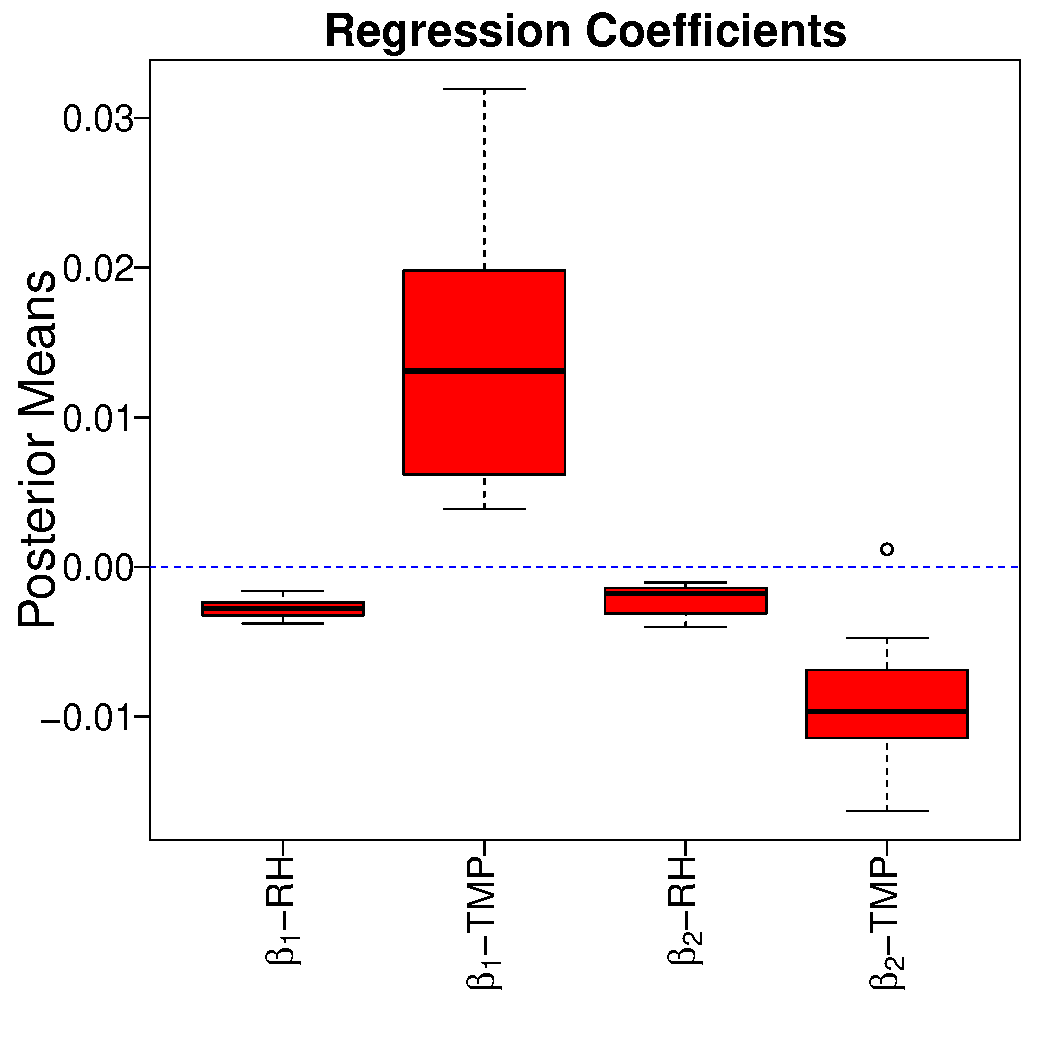
\includegraphics[width=\textwidth]{betas}
      \subcaption{Site-specific regression coefficients}
   \end{subfigure}
     \begin{subfigure}[b]{.35\textwidth}
     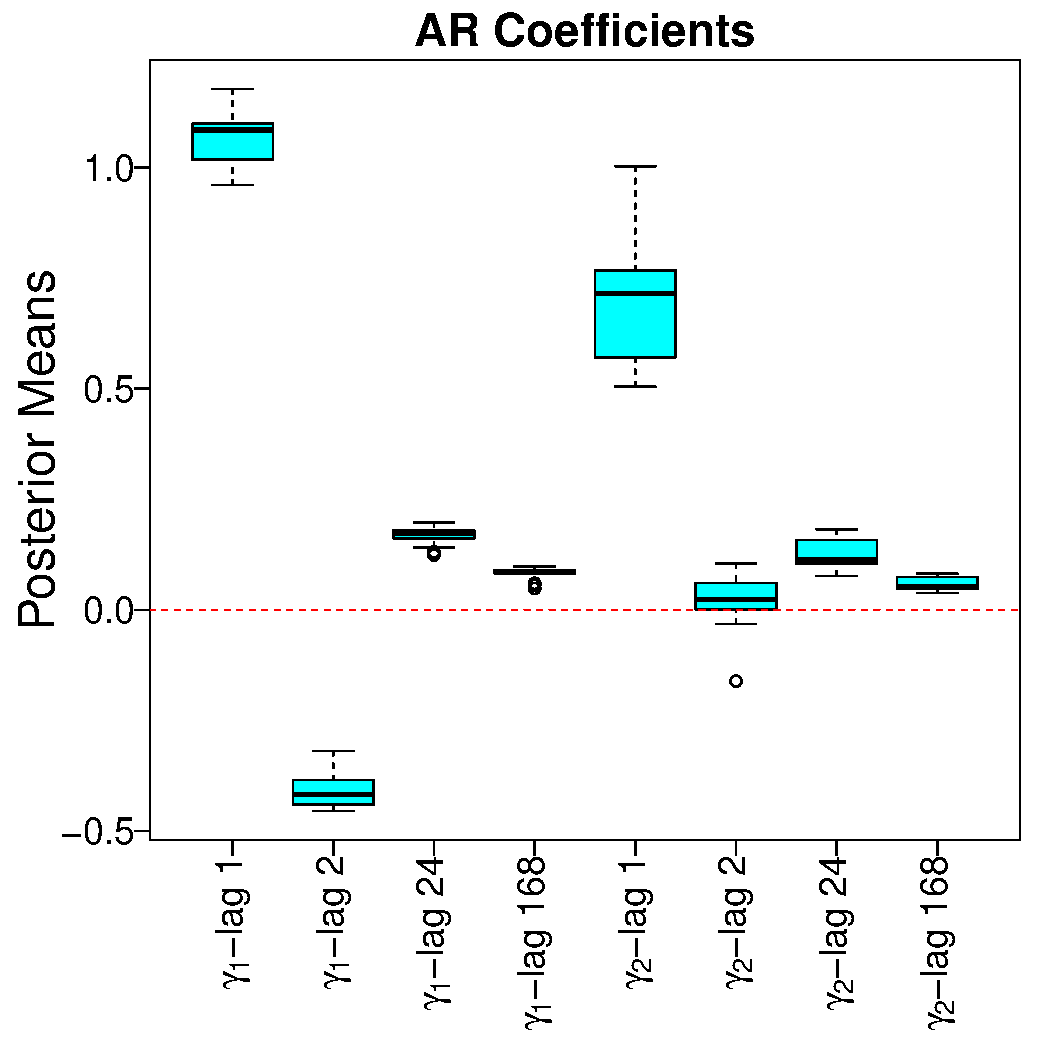
\includegraphics[width=\textwidth]{gammas}
           \subcaption{Site-specific AR coefficients}
   \end{subfigure}
  \end{center}
  \vspace{-4mm}
       \caption{Posterior means for site-specific regression and AR coefficients for ozone and $\text{PM}_{10}$. Each box displays the 24 site-specific posterior means for that coefficient.}\label{fig:post_coef_box}
\end{figure}
\vspace{-6mm}
\begin{figure}[H]
  \begin{center}
   \begin{subfigure}[b]{.35\textwidth}
      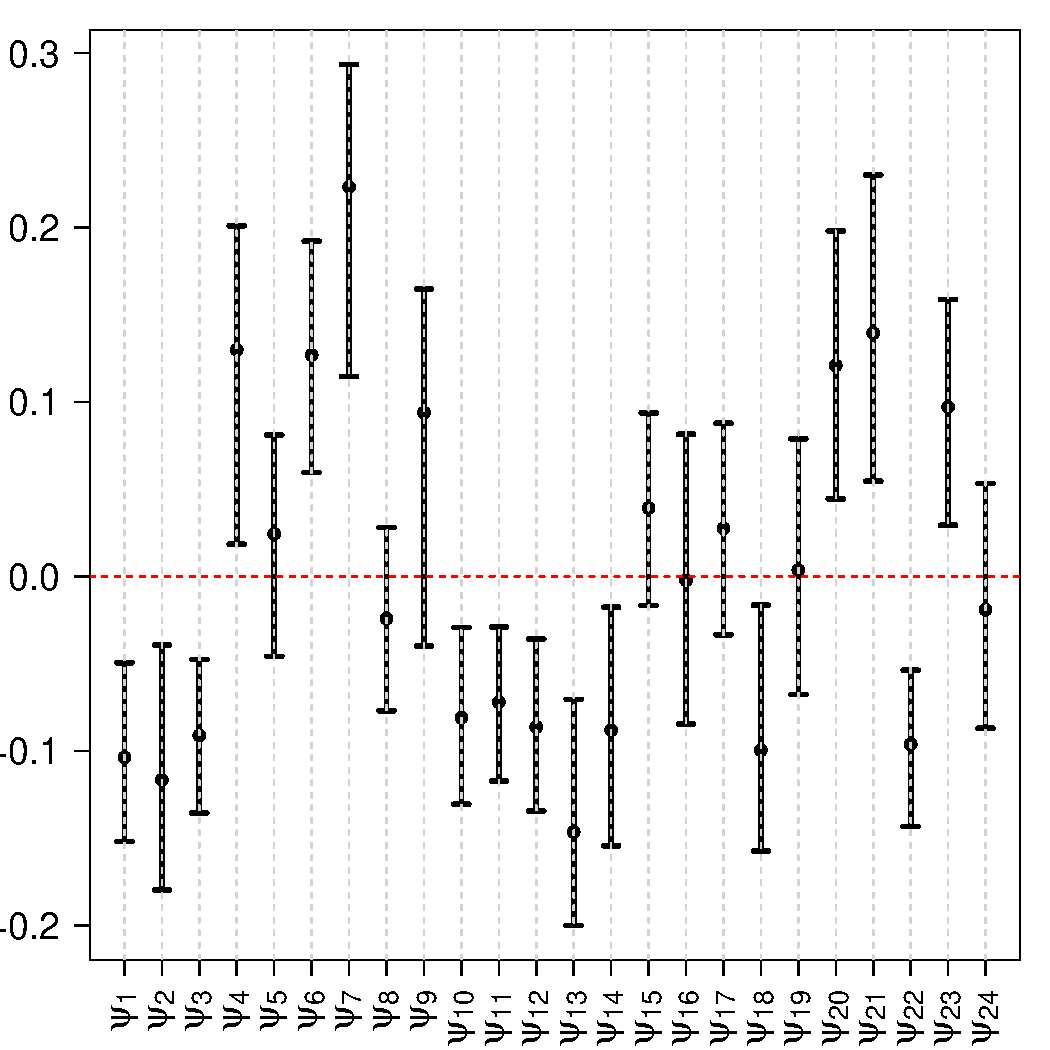
\includegraphics[width=\textwidth]{psi1}
      \subcaption{Site-Specific CAR Effects for Ozone}
   \end{subfigure}
     \begin{subfigure}[b]{.35\textwidth}
     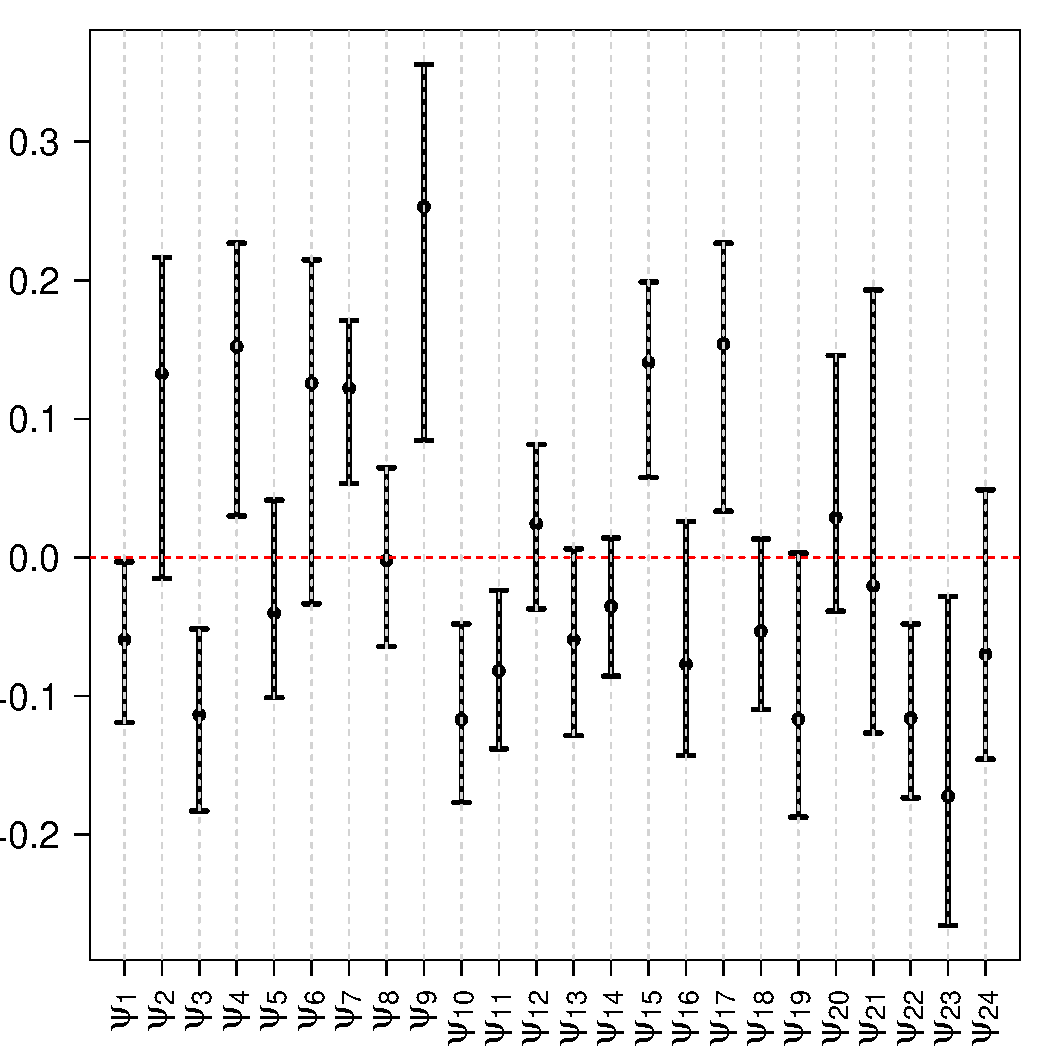
\includegraphics[width=\textwidth]{psi2}
           \subcaption{Site-Specific CAR Effects for $\text{PM}_{10}$}
   \end{subfigure}
  \end{center}
  \vspace{-4mm}
       \caption{Posterior means and credible intervals for site-specific CAR random effects for ozone and $\text{PM}_{10}$. }\label{fig:post_car_box}
\end{figure}

\section{Analysis of Mexican Ambient Air Quality Standards for Illustrative Months}

 For our purposes, we group either type of ozone exceedance, one or eight-hour, together. In the online supplement, we focus on three months, April, August, and December, to illustrate how exceedance probabilities change over the course of the year. April and August are warm months, and ozone creation needs heat. August is the wettest month of the year in Mexico City, on average. Rainfall tends to clear out PM, so $\text{PM}_{10}$ levels are expected to be low in August. April, on the other hand, precedes the rainy season and is normally dry. December is cold and dry. These months naturally contrast each other by illustrating how yearly climate affects pollution levels and the probability of exceeding Mexican ambient air quality standards. We plot regional daily exceedance probabilities for ozone ($P(W_{jd}^O > 95 \text{ ppb} \cup W_{jd}^{\overline{O}} > 70 \text{ ppb})$) and $\text{PM}_{10}$ ($P(W_{jd}^{PM} > 75 \text{ }\mu g / m^3)$) over April (Figure \ref{fig:prob_apr_O3}), August (Figure \ref{fig:prob_aug_O3}), and December (Figure \ref{fig:prob_dec_O3}).  

Recall that April had low phase probabilities except for April 6th when phase I probabilities spiked in all regions due to high ozone levels. Unsurprisingly, the daily exceedance probabilities for ozone are high for all regions in April. The northern regions (NE and NW) have the lowest ozone exceedance probabilities but are still above 1/2 most of the month. Daily $\text{PM}_{10}$ exceedance probabilities vary over the month, with probabilities near one before the 13th, zero from the 13th of April to April 19th, and again high toward the end of the month.

In our phase analysis, we showed that August had uniformly low probabilities of predicted pollution emergencies. Because August is in the rainy season, we expected that it would have low $\text{PM}_{10}$. This is confirmed by our analysis with August having low daily $\text{PM}_{10}$ exceedance probabilities, with the exception of a three days (8/11, 8/15, 8/16). Daily ozone exceedance, on the other hand, is high over most of the month for three regions (CE, SE, SW). Like in April, the northern regions have lower probability of ozone exceedance. 

In December, we showed that phase probabilities were predicted to be low with the exception of a single peak in phase I probabilities in the northeast region due to high $\text{PM}_{10}$ concentrations. Because the phase I $\text{PM}_{10}$ threshold is nearly three times Mexican ambient air quality standards, it is unsurprising to observe high exceedance probabilities for $\text{PM}_{10}$ in the northeast region. It is, however, interesting that four of the five regions have predicted daily exceedance probabilities of one (or very close to one) for 20 or more days. Ozone has many periods of low exceedance probabilities but does exhibit high daily exceedance probabilities overall.
\vspace{-8mm}  
%\textbf{Again, labels on axes are small and regions can be difficult to distinguish.  Again, perhaps multiple panels.  Again, I would remove the horizontal line at .5}
\begin{figure}[H]
  \begin{center}
  \hspace{.1\textwidth}
  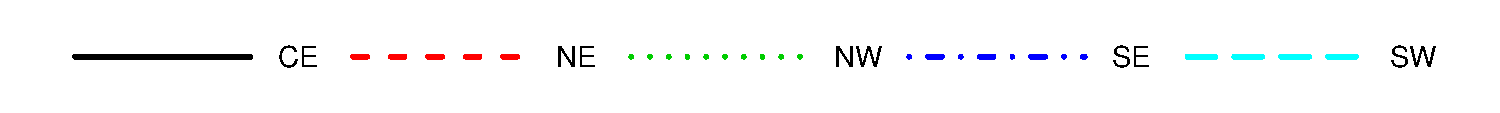
\includegraphics[width=\textwidth]{phase_reg_legend}

  \vspace{-4mm}

      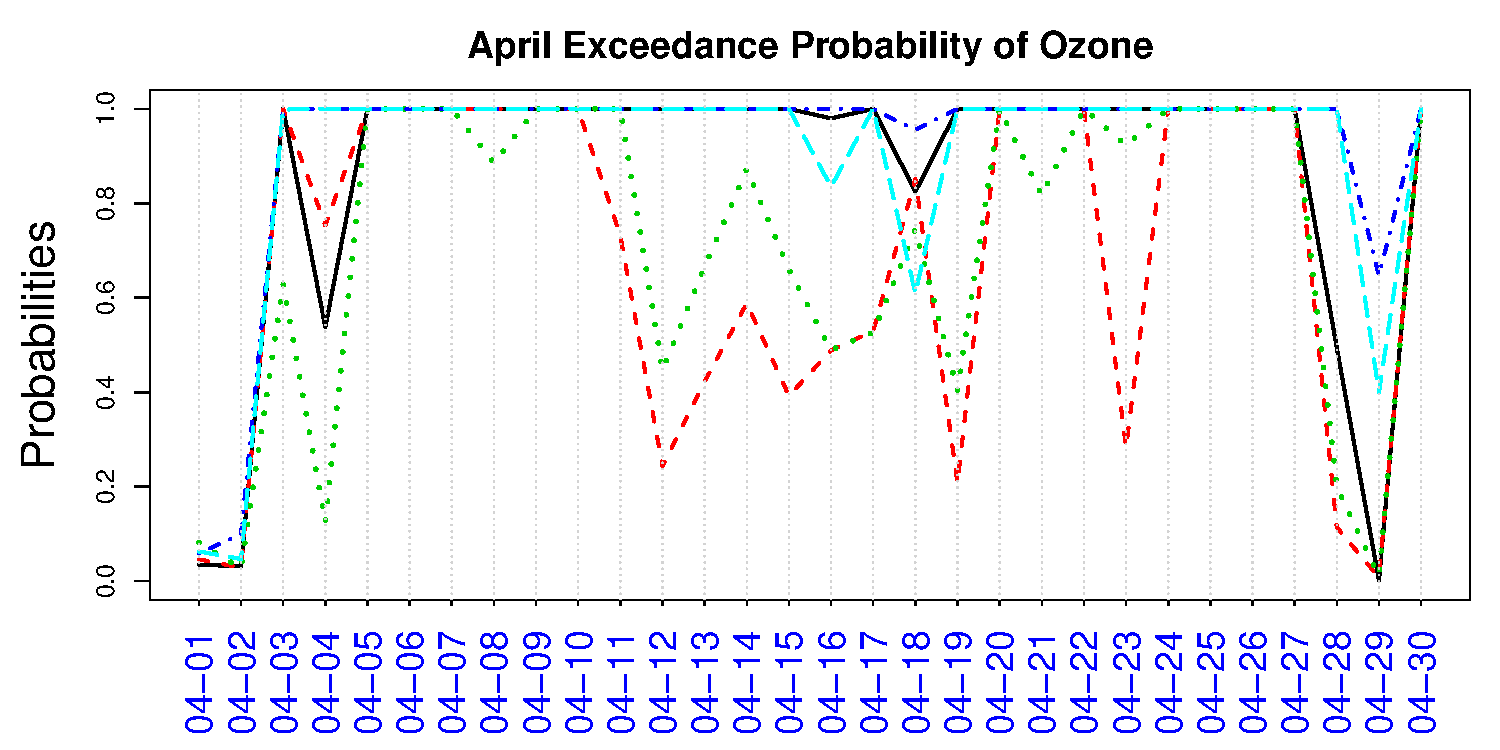
\includegraphics[width=.45\textwidth]{exceed_prob_O3_apr}
            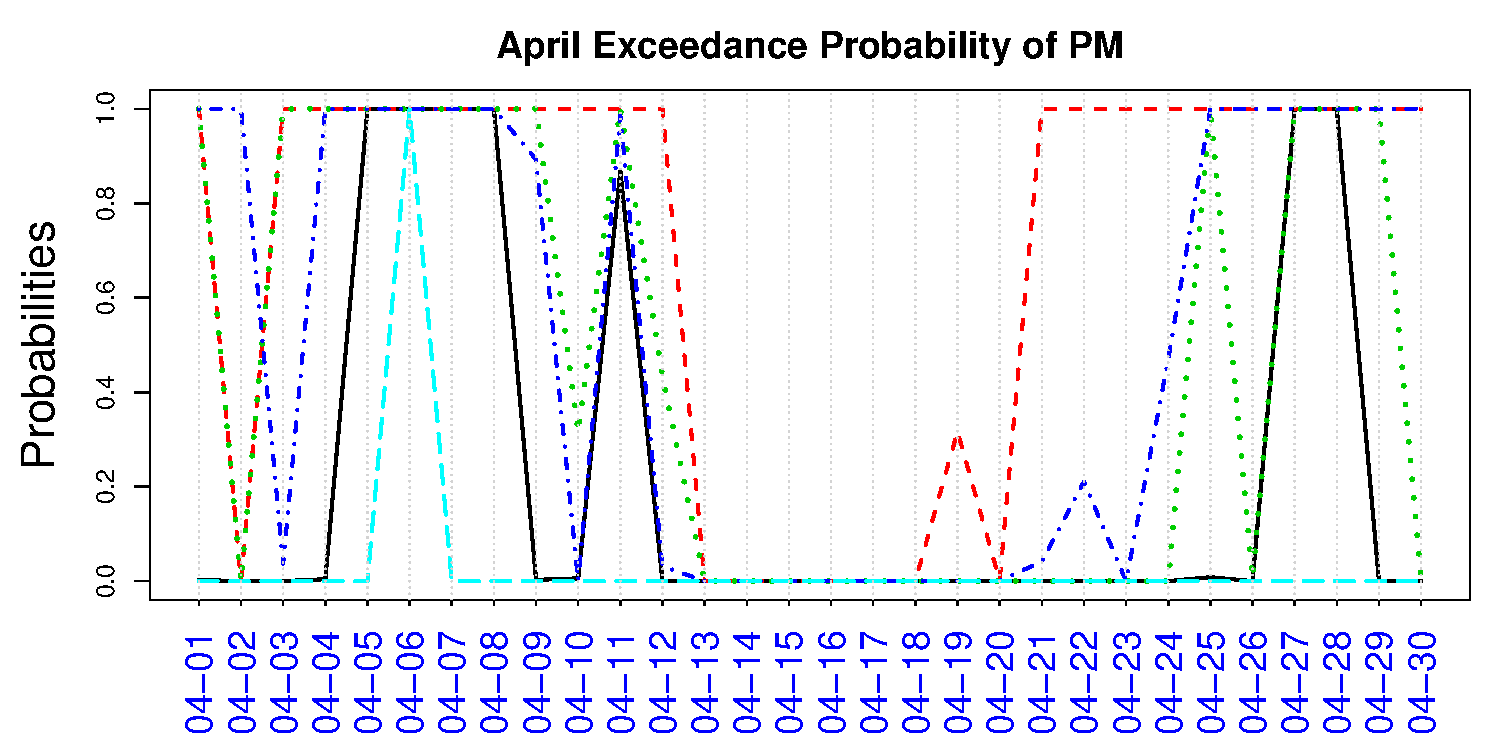
\includegraphics[width=.45\textwidth]{exceed_prob_PM10_apr}

  \end{center}
  \vspace{-6mm}
       \caption{Exceedance probabilities of (Left) ozone and (Right) $\text{PM}_{10}$ for April for each region on a daily level. The colors indicate regions: black represents CE, NE is red, NW is green, SE in blue, and SW is cyan.}\label{fig:prob_apr_O3}
\end{figure}

\vspace{-8mm}  

 \begin{figure}[H]
  \begin{center}
  \hspace{.1\textwidth}
  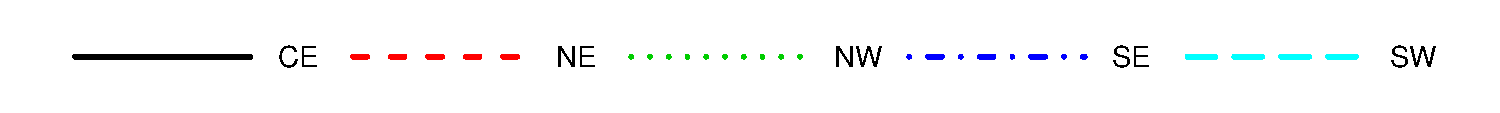
\includegraphics[width=\textwidth]{phase_reg_legend}

  \vspace{-4mm}

      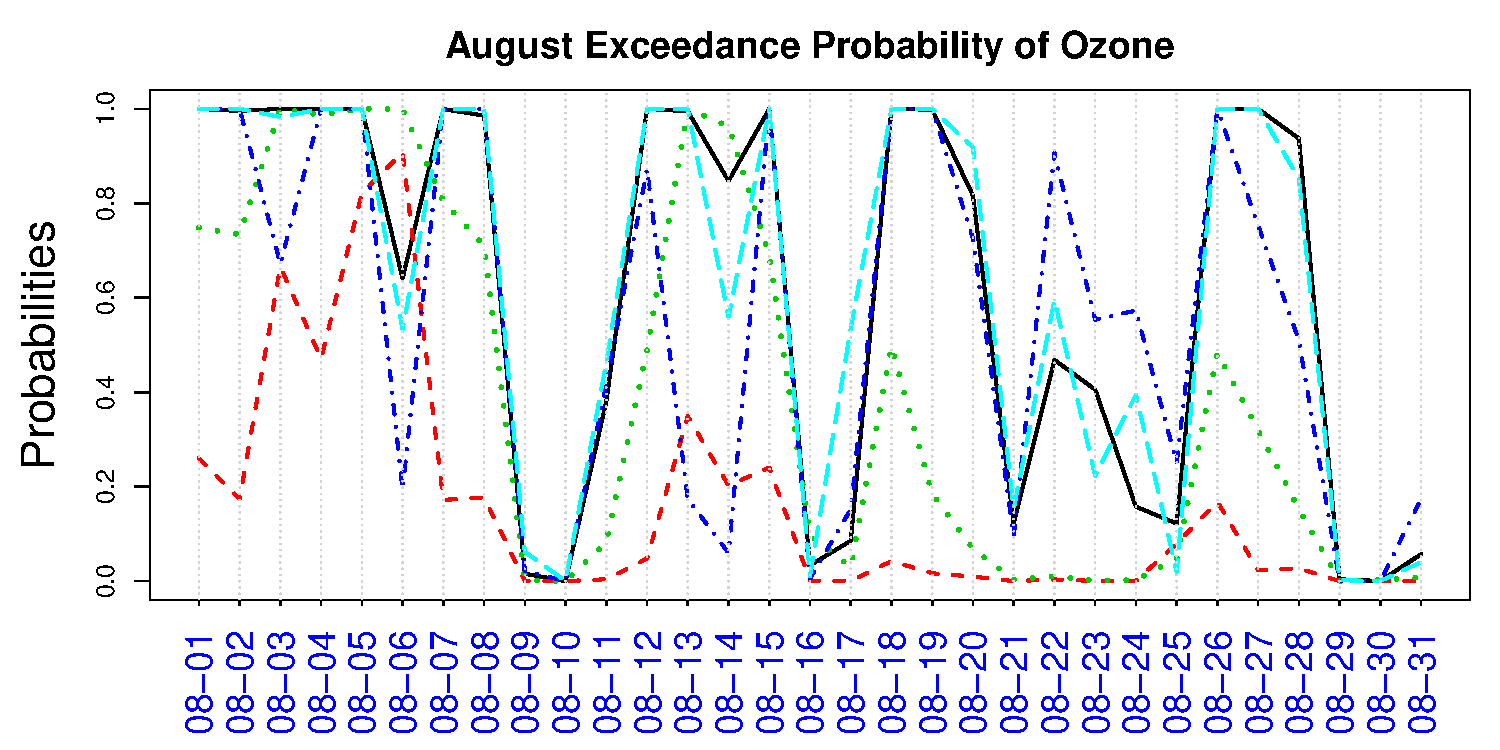
\includegraphics[width=.45\textwidth]{exceed_prob_O3_aug}
      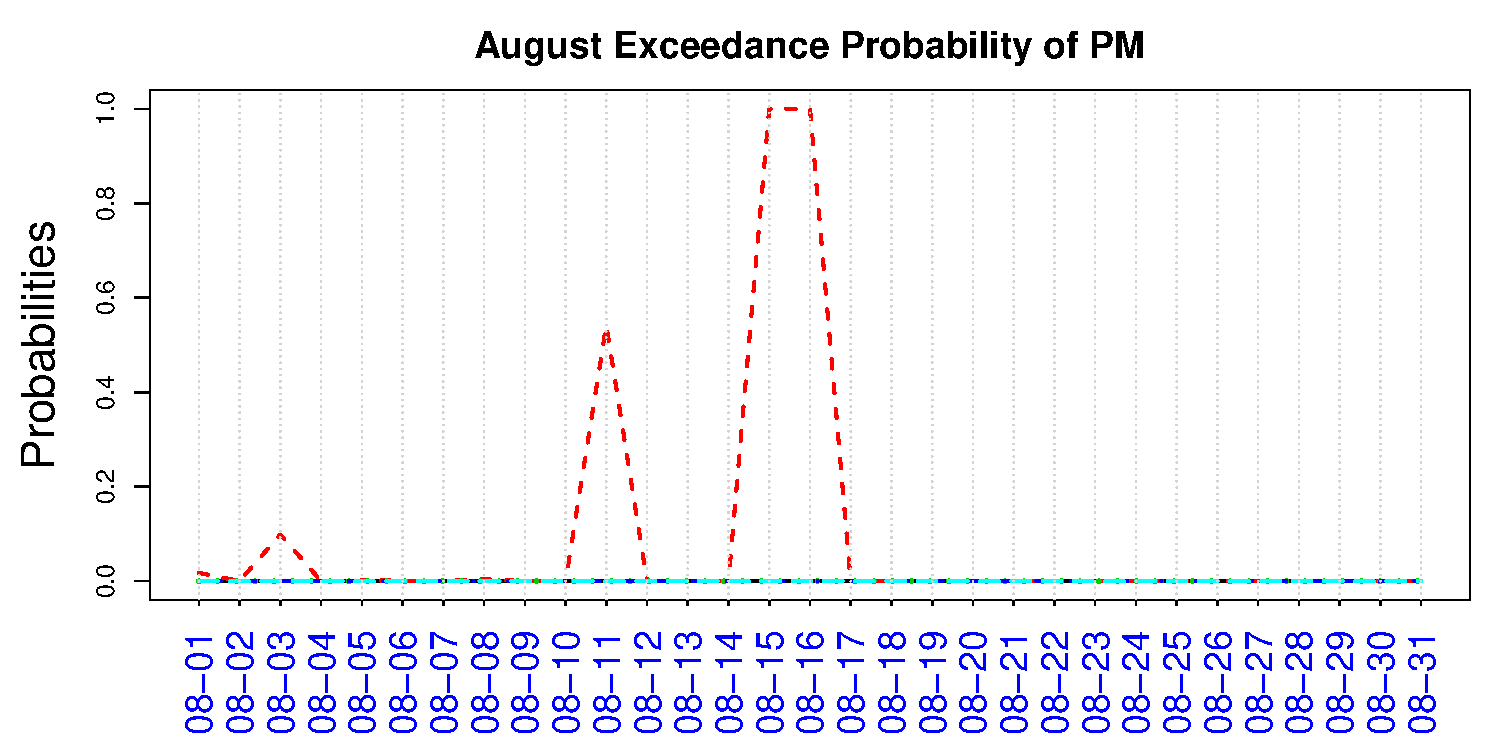
\includegraphics[width=.45\textwidth]{exceed_prob_PM10_aug}

  \end{center}
  \vspace{-6mm}
       \caption{Exceedance probabilities of (Left) ozone and (Right) $\text{PM}_{10}$ for August for each region on a daily level. The colors indicate regions: black represents CE, NE is red, NW is green, SE in blue, and SW is cyan.}\label{fig:prob_aug_O3}
\end{figure}
\vspace{-12mm}  
\begin{figure}[H]
  \begin{center}
  \hspace{.1\textwidth}
  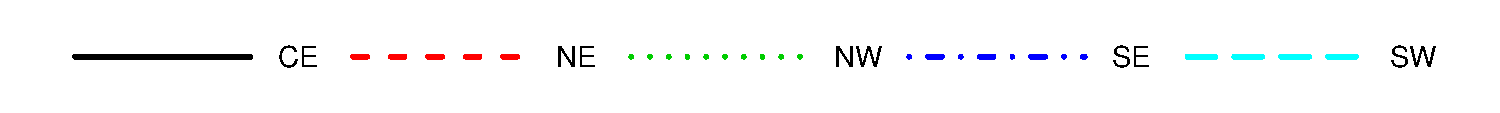
\includegraphics[width=\textwidth]{phase_reg_legend}

  \vspace{-4mm}

      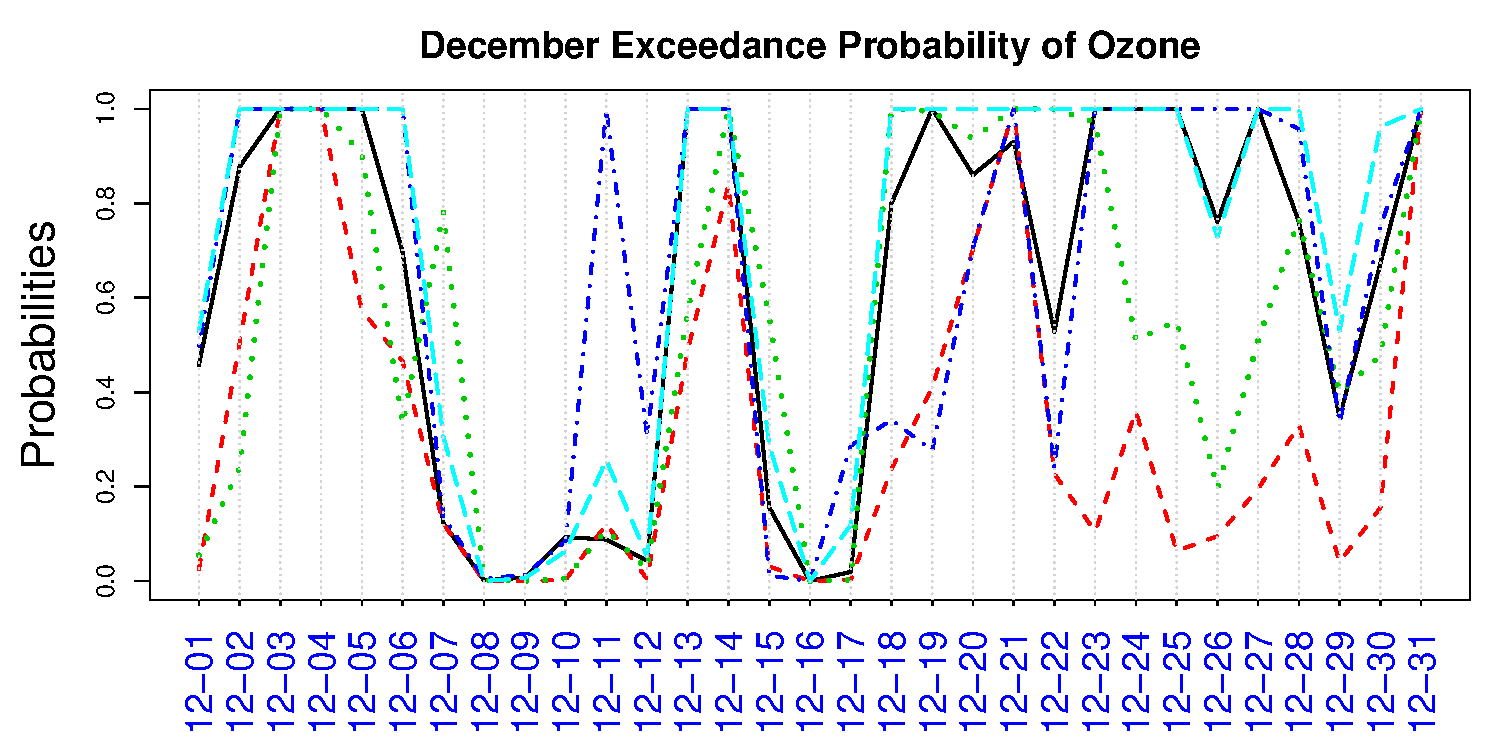
\includegraphics[width=.45\textwidth]{exceed_prob_O3_dec}
            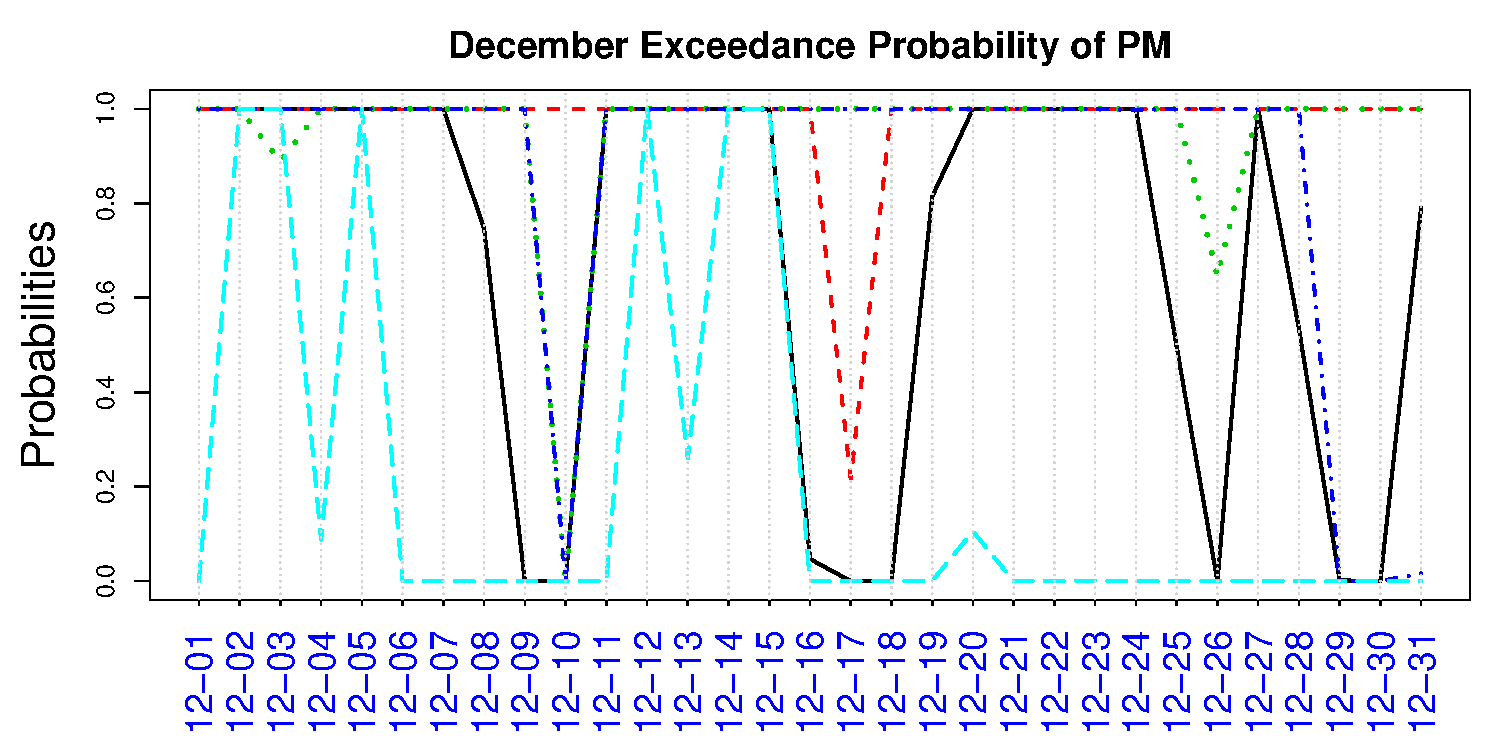
\includegraphics[width=.45\textwidth]{exceed_prob_PM10_dec}


  \end{center}
  \vspace{-6mm}
       \caption{Exceedance probabilities of (Left) ozone and (Right) $\text{PM}_{10}$ for December for each region on a daily level. The colors indicate regions: black represents CE, NE is red, NW is green, SE in blue, and SW is cyan.}\label{fig:prob_dec_O3}
\end{figure}
\vspace{-3mm}  

%\bibliographystyle{rss.bst}
%\bibliographystyle{environmetrics}
\bibliography{refs}

\end{document}
